\documentclass[a4paper]{article}
\usepackage[utf8]{inputenc}
\usepackage{polski}
\usepackage[T1]{fontenc}
\usepackage{amsmath,amssymb,amsthm}
\usepackage{lmodern}
\usepackage[a4paper]{geometry}
\usepackage[dvipsnames]{xcolor}
\usepackage{hyperref}
\usepackage{array}
\usepackage{caption}
\usepackage{tikz}
\usepackage{pgfplots}
\pgfplotsset{compat=1.15}
\usepackage{mathrsfs}
\usetikzlibrary{arrows}

\definecolor{ududff}{rgb}{0.30196078431372547,0.30196078431372547,1.}
\definecolor{xdxdff}{rgb}{0.49019607843137253,0.49019607843137253,1.}
\definecolor{uuuuuu}{rgb}{0.26666666666666666,0.26666666666666666,0.26666666666666666}


% do uzupełnienia
\newcommand{\todo}[1]{\begin{center} \fbox{TODO: #1} \end{center}}

% wyłączenie wcięć
\setlength\parindent{0pt}

% matematyczne
\renewcommand{\mod}{\, \operatorname{mod} \,}
\newcommand{\shift}[2]{\operatorname{shift}_{#2}^{#1}}
\newcommand{\sym}[2]{\operatorname{sym}_{#2}^{#1}}
\newcommand{\id}[1]{\operatorname{id}_{#1}}
\newcommand{\td}{\text{.}}
\newcommand{\tc}{\text{, }}
\newcommand{\floor}[1]{\left\lfloor #1 \right\rfloor}
\newcommand{\twoshift}[1]{\text{TwoShift}_{#1}}
\newcommand{\N}{\mathbb{N}}
\newcommand{\lt}{\left}
\newcommand{\rt}{\right}
\newcommand{\R}{\mathbb{R}}

% twierdzenia, lematy, definicje, fakty, wnioski
\newtheorem{tw}{Twierdzenie}[section]
\newtheorem{lem}[tw]{Lemat}
\theoremstyle{definition}
\newtheorem{df}[tw]{Definicja}
\newtheorem{wn}[tw]{Wniosek}
\newtheorem{fa}[tw]{Fakt}
\newtheorem*{pyt}{Pytanie}

\begin{document}

% ---------- strona tytułowa -----------------

\newpage
\thispagestyle{empty}
\begin{center}
\textbf{\large Uniwersytet Wrocławski\\
Wydział Matematyki i Informatyki\\
Instytut Matematyczny}\\
% \textit{\large specjalność: wpisz tu specjalność}\\
\vspace{4cm}
\textbf{\textit{\large Maksymilian Adamczewski i Jadwiga Świerczyńska}\\
\vspace{0.5cm}
{\Large Sieci przełączników}}\\
\end{center}
\vspace{3cm}
{\large \hspace*{6.5cm}Praca zespołowa\\
\hspace*{6.5cm}napisana pod opieką\\
\hspace*{6.5cm}dr. hab. Jana Dymary, prof. UWr }\\
\vfill
\begin{center}
{\large Wrocław, \the\year{} r.}\\
\end{center}

% -------------- abstrakt ----------------------

\newpage

\null\vfill

\begin{abstract}
    W poniższej pracy przedstawiamy definicje przełącznika oraz sieci przełączników. Najpierw pokazujemy konstrukcje sieci realizujących symetrię, przesunięcie cykliczne czy dowolną permutację. Następnie przedstawiamy konstrukcję sieci Beneša--Waksmana realizującą wszystkie permutacje oraz jej optymalizację. Na końcu konstruujemy sieć realizującą wszystkie przesunięcia cykliczne oraz przesunięcia cykliczne o potęgi 2.  
\end{abstract}

\vfill


% % -------------- spis treści --------------------

% \newpage

\tableofcontents

\newpage


% -------------- wprowadzenie --------------------

\section{Wprowadzenie}

Sieci przełączników to struktury, które można zinterpretować jako urządzenia zbudowane z tzw. \textit{przełączników} pozwalające na permutowanie \(n\) rozróżnialnych sygnałów danych na wejściu. Naturalne jest, że dążymy do optymalizacji struktury sieci pod względem liczby użytych przełączników lub maksymalnej liczby przełączników, przez jakie przepływa sygnał w sieci. Jednakże ze względu na wysoce wyspecjalizowane zastosowania (m. in. sieci telefoniczne, trasowanie pakietów) brakuje źródeł wyczerpująco tłumaczących to zagadnienie w sposób przystępny na przykład dla studenta drugiego roku informatyki. W tej pracy przybliżymy podstawowe definicje (rozdział 2), przedstawimy konstrukcję najsłynniejszej sieci realizującej wszystkie permutacje, czyli sieci Beneša--Waksmana (rozdział 3), sieci realizującej wszystkie przesunięcia cykliczne (rozdział 4) i sieci realizującej przesunięcia cykliczne o potęgi 2 (rozdział 5).  
% Natomiast w rozdziale 6 przeanalizujemy sieci, w których przełączniki są ustawiane losowo w jeden z dwóch stanów. 

\vspace{1em}

Zastrzegamy jednak, że za względu na cel pracy, polegający na przystępnym przybliżeniu tematu, przy formułowaniu definicji i konstrukcji będziemy skupiać się na intuicji. Precyzyjną matematyczną formalizację pozostawimy jako ćwiczenie dla Czytelnika, które okaże się schematycznym zadaniem, gdy już się zrozumie idee stojące za sieciami przełączników. 

\vspace{1em}

Przez \(S_n\) będziemy oznaczać zbiór wszystkich permutacji \(\{0, 1, \ldots, n-1\}\), przez
\[
\shift{n}{k} : \{0, 1, \ldots, n-1\} \to \{0, 1, \ldots, n-1\} 
\]
permutację \(\shift{n}{k}(i) = (k+i) \mod n\), a przez
\[
\sym{n}{k} : \{0, 1, \ldots, n-1\} \to \{0, 1, \ldots, n-1\} 
\]
permutację \(\sym{n}{k}(i) = (k-i) \mod n\), natomiast przez 
\[
\id{n} : \{0, 1, \ldots, n-1\} \to \{0, 1, \ldots, n-1\} 
\]
permutację identycznościową. 

\vspace{1em}

Ponadto stosujemy następujące oznaczenia złożoności asymptotycznej (podobnie jak w \cite{cormen}).

\begin{df}
    Dla danych funkcji \(f, g : \N \to \R\) mówimy, że:
    \begin{itemize}
        \item \(f = O(g)\), gdy istnieją \( n_0 \in \N, \,  c > 0\), takie że 
        \[
            0 \leq f(n) \leq cg(n)  \text{ dla wszystkich } n \geq n_0 \tc
        \]
        \item \(f = \Omega(g)\), gdy istnieją \( n_0 \in \N, \,  c > 0\), takie że 
        \[
            0 \leq cg(n) \leq f(n)  \text{ dla wszystkich } n \geq n_0 \tc
        \]
        \item  \(f = \Theta(g)\), gdy istnieją \( n_0 \in \N, \,  c_1 > 0, c_2 > 0\), takie że 
        \[
            0 \leq c_1 g(n) \leq f(n) \leq c_2 g(n)  \text{ dla wszystkich } n \geq n_0 \td
        \]
    \end{itemize}
\end{df}


% -------- podstawowe definicje i fakty -----------

\section{Podstawy}

\subsection{Definicje}

Zacznijmy od najistotniejszej dla tej pracy kwestii -- czyli definicji przełącznika.

\vspace{1em}

{\bf Przełącznikiem} nazywamy urządzenie mające dwa wejścia (oznaczone liczbami 0 i 1)  i dwa wyjścia (oznaczone liczbami 0 i 1). Może się znaleźć w dwóch stanach:

\begin{itemize}
    \item nieaktywnym -- sygnał z wejścia \(i\) trafia do wyjścia \(i\) (dla \(i \in \{0,1\}\)),
    \item  aktywnym -- sygnał z wejścia \(i\) trafia do wyjścia \((i+1) \mod 2\) (dla \(i \in \{0,1\}\)).
\end{itemize}

\begin{center}
    \begin{minipage}{.5\textwidth} %
        \begin{center}
            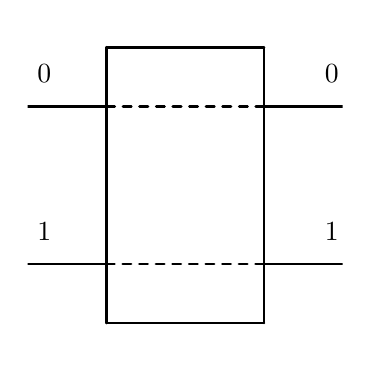
\begin{tikzpicture}[line cap=round,line join=round,>=triangle 45,x=0.5cm,y=0.5cm]
            \clip(-2,-1.) rectangle (6.,7.5);
            \draw [line width=1.pt] (0.,0.)-- (4.,0.);
            \draw [line width=1.pt] (4.,0.)-- (4.,7.);
            \draw [line width=1.pt] (4.,7.)-- (0.,7.);
            \draw [line width=1.pt] (0.,7.)-- (0.,0.);
            \draw (-2.,6.8) node[anchor=north west] {0};
            \draw (5.3,6.8) node[anchor=north west] {0};
            \draw (-2.,2.8) node[anchor=north west] {1};
            \draw (5.3,2.8) node[anchor=north west] {1};
            \draw [line width=1.pt] (0.,5.5)-- (-2.,5.5);
            \draw [line width=1.pt] (4.,5.5)-- (6.,5.5);
            \draw [line width=1.pt] (0.,1.5)-- (-2.,1.5);
            \draw [line width=1.pt] (4.,1.5)-- (6.,1.5);
            \draw [line width=1.pt, dashed] (4.,1.5)-- (0.,1.5);
            \draw [line width=1.pt, dashed] (0.,5.5)-- (4.,5.5);
            \end{tikzpicture}
            
            {\it Przełącznik w stanie nieaktywnym}
        \end{center}
        
    \end{minipage}%
    \begin{minipage}{.5\textwidth} %
        \begin{center} 
            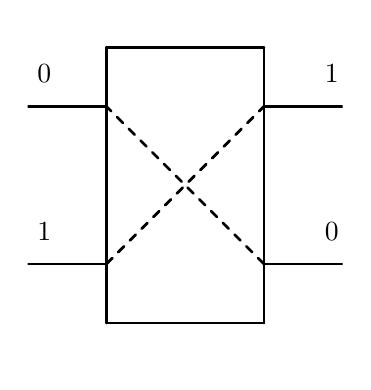
\begin{tikzpicture}[line cap=round,line join=round,>=triangle 45,x=0.5cm,y=0.5cm]
            \clip(-2,-1.) rectangle (6.,7.5);
            \draw [line width=1.pt] (0.,0.)-- (4.,0.);
            \draw [line width=1.pt] (4.,0.)-- (4.,7.);
            \draw [line width=1.pt] (4.,7.)-- (0.,7.);
            \draw [line width=1.pt] (0.,7.)-- (0.,0.);
            \draw (-2.,6.8) node[anchor=north west] {0};
            \draw (5.3,6.8) node[anchor=north west] {1};
            \draw (-2.,2.8) node[anchor=north west] {1};
            \draw (5.3,2.8) node[anchor=north west] {0};
            \draw [line width=1.pt] (0.,5.5)-- (-2.,5.5);
            \draw [line width=1.pt] (4.,5.5)-- (6.,5.5);
            \draw [line width=1.pt] (0.,1.5)-- (-2.,1.5);
            \draw [line width=1.pt] (4.,1.5)-- (6.,1.5);
            \draw [line width=1.pt, dashed] (4.,1.5)-- (0.,5.5);
            \draw [line width=1.pt, dashed] (0.,1.5)-- (4.,5.5);
            \end{tikzpicture}

            {\it Przełącznik w stanie aktywnym}
        \end{center}
    \end{minipage} 
\end{center}

\vspace{1em}

Przełączniki w naturalny sposób możemy ze sobą łączyć {\bf przewodami} -- sygnał z wyjścia jednego przełącznika może zostać przekierowany przewodem na wejście innego przełącznika. 

\vspace{1em}

Połączone przewodniki tworzą {\bf sieć przełączników}. Dokładniej, siecią przełączników o \(n\) wejściach i \(n\) wyjściach nazywamy zbiór przełączników i przewodów, w którym:

\begin{itemize}
    \item z każdego wyjścia przełącznika w sieci wychodzi dokładnie jeden przewód,
    \item do każdego wejścia przełącznika w sieci wchodzi dokładnie jeden przewód,
    \item z każdego wejścia sieci wychodzi dokładnie jeden przewód,
    \item  do każdego wyjścia sieci wchodzi dokładnie jeden przewód, 
    \item żaden przewód nie jest podłączony dwoma końcami do tego samego przełącznika,
    \item wejście każdego przewodu jest wpięte do wyjścia pewnego przełącznika lub do wejścia sieci,
    \item wyjście każdego przewodu jest wpięte do wejścia pewnego przełącznika lub do wyjścia sieci,
    \item mamy \(n\) wejść i \(n\) wyjść sieci.
\end{itemize}

Ponadto wejścia i wyjścia sieci numerujemy liczbami od \(0\) do \(n-1\).


\begin{minipage}{.5\textwidth}
\begin{center}

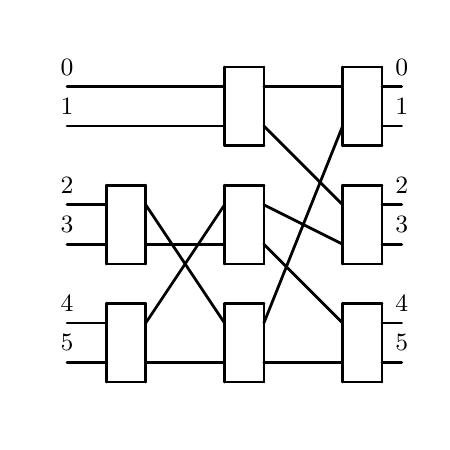
\begin{tikzpicture}[line cap=round,line join=round,>=triangle 45,x=0.5cm,y=0.5cm]
\clip(-2.,-1.) rectangle (8.,9.);

\draw (-1.,8.) node {\small 0};
\draw (-1.,7.) node {\small 1};
\draw (-1.,5.) node {\small 2};
\draw (-1.,4.) node {\small 3};
\draw (-1.,2.) node {\small 4};
\draw (-1.,1.) node {\small 5};

\draw (7.5,8.) node {\small 0};
\draw (7.5,7.) node {\small 1};
\draw (7.5,5.) node {\small 2};
\draw (7.5,4.) node {\small 3};
\draw (7.5,2.) node {\small 4};
\draw (7.5,1.) node {\small 5};
% \draw (-1.,4.) node[anchor=north west] {1};
% \draw (-1.,3.) node[anchor=north west] {2};
% \draw (-1.,2.) node[anchor=north west] {3};
% \draw (-1.,1.) node[anchor=north west] {3};
% \draw (-1.,0.) node[anchor=north west] {3};

\draw [line width=1.pt] (0.,0.)-- (1.,0.);
\draw [line width=1.pt] (1.,2.)-- (1.,0.);
\draw [line width=1.pt] (1.,2.)-- (0.,2.);
\draw [line width=1.pt] (0.,0.)-- (0.,2.);
\draw [line width=1.pt] (0.,3.)-- (1.,3.);
\draw [line width=1.pt] (1.,3.)-- (1.,5.);
\draw [line width=1.pt] (1.,5.)-- (0.,5.);
\draw [line width=1.pt] (0.,3.)-- (0.,5.);
\draw [line width=1.pt] (3.,8.)-- (3.,6.);
\draw [line width=1.pt] (3.,6.)-- (4.,6.);
\draw [line width=1.pt] (4.,6.)-- (4.,8.);
\draw [line width=1.pt] (4.,8.)-- (3.,8.);
\draw [line width=1.pt] (3.,5.)-- (3.,3.);
\draw [line width=1.pt] (3.,3.)-- (4.,3.);
\draw [line width=1.pt] (4.,3.)-- (4.,5.);
\draw [line width=1.pt] (4.,5.)-- (3.,5.);
\draw [line width=1.pt] (3.,2.)-- (3.,0.);
\draw [line width=1.pt] (3.,0.)-- (4.,0.);
\draw [line width=1.pt] (4.,0.)-- (4.,2.);
\draw [line width=1.pt] (4.,2.)-- (3.,2.);
\draw [line width=1.pt] (6.,8.)-- (6.,6.);
\draw [line width=1.pt] (6.,6.)-- (7.,6.);
\draw [line width=1.pt] (7.,6.)-- (7.,8.);
\draw [line width=1.pt] (7.,8.)-- (6.,8.);
\draw [line width=1.pt] (6.,5.)-- (6.,3.);
\draw [line width=1.pt] (6.,3.)-- (7.,3.);
\draw [line width=1.pt] (7.,3.)-- (7.,5.);
\draw [line width=1.pt] (7.,5.)-- (6.,5.);
\draw [line width=1.pt] (6.,2.)-- (6.,0.);
\draw [line width=1.pt] (6.,0.)-- (7.,0.);
\draw [line width=1.pt] (7.,0.)-- (7.,2.);
\draw [line width=1.pt] (7.,2.)-- (6.,2.);

\draw [line width=1.pt] (0.,4.5)-- (-1.,4.5);
\draw [line width=1.pt] (0.,3.5)-- (-1.,3.5);
\draw [line width=1.pt] (0.,1.5)-- (-1.,1.5);
\draw [line width=1.pt] (0.,0.5)-- (-1.,0.5);
\draw [line width=1.pt] (3.,7.5)-- (-1.,7.5);
\draw [line width=1.pt] (3.,6.5)-- (-1.,6.5);

\draw [line width=1.pt] (1.,4.5)-- (3.,1.5);
\draw [line width=1.pt] (1.,3.5)-- (3.,3.5);
\draw [line width=1.pt] (1.,1.5)-- (3.,4.5);
\draw [line width=1.pt] (1.,0.5)-- (3.,0.5);
\draw [line width=1.pt] (4.,1.5)-- (6.,6.5);
\draw [line width=1.pt] (4.,7.5)-- (6.,7.5);
\draw [line width=1.pt] (4.,6.5)-- (6.,4.5);
\draw [line width=1.pt] (4.,4.5)-- (6.,3.5);
\draw [line width=1.pt] (4.,3.5)-- (6.,1.5);
\draw [line width=1.pt] (4.,0.5)-- (6.,0.5);
\draw [line width=1.pt] (7.,7.5)-- (7.5,7.5);
\draw [line width=1.pt] (7.,6.5)-- (7.5,6.5);
\draw [line width=1.pt] (7.,4.5)-- (7.5,4.5);
\draw [line width=1.pt] (7.,3.5)-- (7.5,3.5);
\draw [line width=1.pt] (7.,1.5)-- (7.5,1.5);
\draw [line width=1.pt] (7.,0.5)-- (7.5,0.5);
\end{tikzpicture}

% {\it Przykład sieci przełączników}
\end{center} 
\end{minipage}
\begin{minipage}{.5\textwidth}
\begin{center}
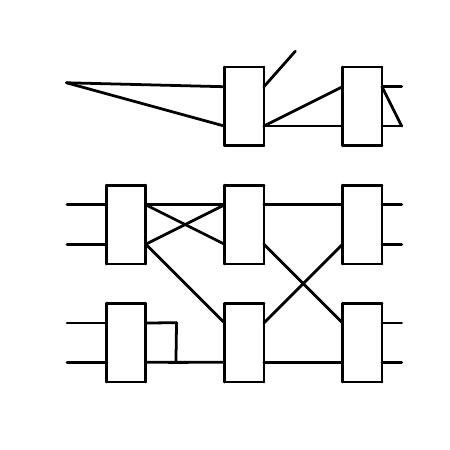
\begin{tikzpicture}[line cap=round,line join=round,>=triangle 45,x=0.5cm,y=0.5cm]
\clip(-2.,-1.) rectangle (8.,9.);
\draw [line width=1.pt] (0.,0.)-- (1.,0.);
\draw [line width=1.pt] (1.,2.)-- (1.,0.);
\draw [line width=1.pt] (1.,2.)-- (0.,2.);
\draw [line width=1.pt] (0.,0.)-- (0.,2.);
\draw [line width=1.pt] (0.,3.)-- (1.,3.);
\draw [line width=1.pt] (1.,3.)-- (1.,5.);
\draw [line width=1.pt] (1.,5.)-- (0.,5.);
\draw [line width=1.pt] (0.,3.)-- (0.,5.);
\draw [line width=1.pt] (3.,8.)-- (3.,6.);
\draw [line width=1.pt] (3.,6.)-- (4.,6.);
\draw [line width=1.pt] (4.,6.)-- (4.,8.);
\draw [line width=1.pt] (4.,8.)-- (3.,8.);
\draw [line width=1.pt] (3.,5.)-- (3.,3.);
\draw [line width=1.pt] (3.,3.)-- (4.,3.);
\draw [line width=1.pt] (4.,3.)-- (4.,5.);
\draw [line width=1.pt] (4.,5.)-- (3.,5.);
\draw [line width=1.pt] (3.,2.)-- (3.,0.);
\draw [line width=1.pt] (3.,0.)-- (4.,0.);
\draw [line width=1.pt] (4.,0.)-- (4.,2.);
\draw [line width=1.pt] (4.,2.)-- (3.,2.);
\draw [line width=1.pt] (6.,8.)-- (6.,6.);
\draw [line width=1.pt] (6.,6.)-- (7.,6.);
\draw [line width=1.pt] (7.,6.)-- (7.,8.);
\draw [line width=1.pt] (7.,8.)-- (6.,8.);
\draw [line width=1.pt] (6.,5.)-- (6.,3.);
\draw [line width=1.pt] (6.,3.)-- (7.,3.);
\draw [line width=1.pt] (7.,3.)-- (7.,5.);
\draw [line width=1.pt] (7.,5.)-- (6.,5.);
\draw [line width=1.pt] (6.,2.)-- (6.,0.);
\draw [line width=1.pt] (6.,0.)-- (7.,0.);
\draw [line width=1.pt] (7.,0.)-- (7.,2.);
\draw [line width=1.pt] (7.,2.)-- (6.,2.);
\draw [line width=1.pt] (0.,4.5)-- (-1.,4.5);
\draw [line width=1.pt] (0.,3.5)-- (-1.,3.5);
\draw [line width=1.pt] (0.,1.5)-- (-1.,1.5);
\draw [line width=1.pt] (0.,0.5)-- (-1.,0.5);
\draw [line width=1.pt] (7.,7.5)-- (7.5,7.5);
\draw [line width=1.pt] (7.,6.5)-- (7.5,6.5);
\draw [line width=1.pt] (7.,4.5)-- (7.5,4.5);
\draw [line width=1.pt] (7.,3.5)-- (7.5,3.5);
\draw [line width=1.pt] (7.,1.5)-- (7.5,1.5);
\draw [line width=1.pt] (7.,0.5)-- (7.5,0.5);
\draw [line width=1.pt] (1.,4.5)-- (3.,4.5);
\draw [line width=1.pt] (1.,4.5)-- (3.,3.5);
\draw [line width=1.pt] (1.,3.5)-- (3.,4.5);
\draw [line width=1.pt] (1.,1.5)-- (1.7813908792453008,1.5039475958137278);
\draw [line width=1.pt] (1.7813908792453008,1.5039475958137278)-- (1.7656781783217494,0.4983347367064437);
\draw [line width=1.pt] (1.7656781783217494,0.4983347367064437)-- (1.,0.5);
\draw [line width=1.pt] (-1.0154698851468411,7.600475554151638)-- (3.,6.5);
\draw [line width=1.pt] (-1.0154698851468411,7.600475554151638)-- (3.,7.5);
\draw [line width=1.pt] (4.,7.5)-- (4.798229456567162,8.401823301252755);
\draw [line width=1.pt] (4.,6.5)-- (6.,7.5);
\draw [line width=1.pt] (4.,6.5)-- (6.,6.5);
\draw [line width=1.pt] (4.,4.5)-- (6.,4.5);
\draw [line width=1.pt] (3.,1.5)-- (1.,3.5);
\draw [line width=1.pt] (3.,0.5)-- (1.7656781783217494,0.4983347367064437);
\draw [line width=1.pt] (4.,3.5)-- (6.,1.5);
\draw [line width=1.pt] (4.,1.5)-- (6.,3.5);
\draw [line width=1.pt] (4.,0.5)-- (6.,0.5);
\draw [line width=1.pt] (7.,7.5)-- (7.5,6.5);
\end{tikzpicture}

% {\it Przykład przełączników połączonych przewodami, które nie tworzą sieci przełączników}
\end{center} 
\end{minipage}

\begin{minipage}{.5\textwidth}
    \begin{center}
        {\it Przykład sieci przełączników}
    \end{center}
\end{minipage}
\begin{minipage}{.5\textwidth}
    \begin{center}
        {\it Przykład przełączników połączonych przewodami, które nie tworzą sieci przełączników}
    \end{center}
\end{minipage}




\begin{df}
    Mówimy, że sieć przełączników o \(n\) wejściach i \(n\) wyjściach realizuje permutację \(\sigma \in S_n\), gdy każdemu przewodnikowi możemy nadać stan (aktywny lub nieaktywny) tak, by dla sygnałów w kolejności \(0, 1, \ldots, n-1\) na wejściu otrzymać sygnały w kolejności \(\sigma (0), \sigma (1), \ldots, \sigma (n-1)\) na wyjściu. 
\end{df}

Poniższa sieć wraz z przedstawionymi stanami przełączników realizuje permutację

\[
    \begin{pmatrix}
        0 & 1 & 2 & 3 & 4  \\
        1 & 0 & 4 & 3 & 2 
    \end{pmatrix} 
\]

(liczby znajdujące się przy wyjściach tej sieci nie są numerami wyjść, lecz numerami wejść, z których pochodzą sygnały trafiające do nich).

\begin{center}
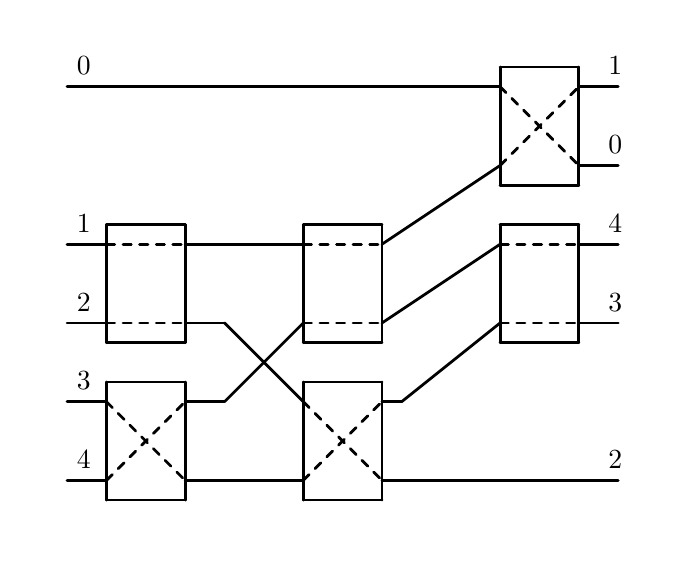
\begin{tikzpicture}[line cap=round,line join=round,>=triangle 45,x=0.5cm,y=0.5cm]
\clip(-2.,-1.) rectangle (14.,12.);
\draw [line width=1.pt] (0.,0.)-- (2.,0.);
\draw [line width=1.pt] (2.,0.)-- (2.,3.);
\draw [line width=1.pt] (2.,3.)-- (0.,3.);
\draw [line width=1.pt] (0.,3.)-- (0.,0.);
\draw [line width=1.pt] (0.,4.)-- (2.,4.);
\draw [line width=1.pt] (2.,4.)-- (2.,7.);
\draw [line width=1.pt] (2.,7.)-- (0.,7.);
\draw [line width=1.pt] (0.,7.)-- (0.,4.);
\draw [line width=1.pt] (5.,3.)-- (7.,3.);
\draw [line width=1.pt] (7.,3.)-- (7.,0.);
\draw [line width=1.pt] (7.,0.)-- (5.,0.);
\draw [line width=1.pt] (5.,0.)-- (5.,3.);
\draw [line width=1.pt] (5.,4.)-- (7.,4.);
\draw [line width=1.pt] (7.,4.)-- (7.,7.);
\draw [line width=1.pt] (7.,7.)-- (5.,7.);
\draw [line width=1.pt] (5.,7.)-- (5.,4.);
\draw [line width=1.pt] (10.,4.)-- (12.,4.);
\draw [line width=1.pt] (12.,4.)-- (12.,7.);
\draw [line width=1.pt] (12.,7.)-- (10.,7.);
\draw [line width=1.pt] (10.,7.)-- (10.,4.);
\draw [line width=1.pt] (10.,8.)-- (12.,8.);
\draw [line width=1.pt] (12.,8.)-- (12.,11.);
\draw [line width=1.pt] (12.,11.)-- (10.,11.);
\draw [line width=1.pt] (10.,11.)-- (10.,8.);
\draw [line width=1.pt] (0.,2.5)-- (-1.,2.5);
\draw [line width=1.pt] (2.,2.5)-- (3.,2.5);
\draw [line width=1.pt] (2.,0.5)-- (3.,0.5);
\draw [line width=1.pt] (0.,0.5)-- (-1.,0.5);
\draw [line width=1.pt] (0.,4.5)-- (-1.,4.5);
\draw [line width=1.pt] (2.,4.5)-- (3.,4.5);
\draw [line width=1.pt] (0.,6.5)-- (-1.,6.5);
\draw [line width=1.pt] (2.,6.5)-- (3.,6.5);
\draw [line width=1.pt, dashed] (0.,6.5)-- (2.,6.5);
\draw [line width=1.pt, dashed] (0.,4.5)-- (2.,4.5);
\draw [line width=1.pt, dashed] (0.,2.5)-- (2.,0.5);
\draw [line width=1.pt, dashed] (0.,0.5)-- (2.,2.5);
\draw [line width=1.pt] (3.,2.5)-- (5.,4.5);
\draw [line width=1.pt] (3.,4.5)-- (5.,2.5);
\draw [line width=1.pt] (3.,0.5)-- (5.,0.5);
\draw [line width=1.pt] (3.,6.5)-- (5.,6.5);
\draw [line width=1.pt] (7.,2.5)-- (7.5,2.5);
\draw [line width=1.pt] (7.,0.5)-- (7.5,0.5);
\draw [line width=1.pt] (7.5,0.5)-- (13.,0.5);
\draw [line width=1.pt] (7.5,2.5)-- (10.,4.5);
\draw [line width=1.pt, dashed] (5.,2.5)-- (7.,0.5);
\draw [line width=1.pt, dashed] (5.,0.5)-- (7.,2.5);
\draw [line width=1.pt] (7.,4.5)-- (10.,6.5);
\draw [line width=1.pt] (7.,6.5)-- (10.,8.5);
\draw [line width=1.pt] (10.,10.5)-- (-1.,10.5);
\draw [line width=1.pt] (12.,6.5)-- (13.,6.5);
\draw [line width=1.pt] (12.,4.5)-- (13.,4.5);
\draw [line width=1.pt] (12.,10.5)-- (13.,10.5);
\draw [line width=1.pt] (12.,8.5)-- (13.,8.5);
\draw [line width=1.pt, dashed] (10.,10.5)-- (12.,8.5);
\draw [line width=1.pt, dashed] (10.,8.5)-- (12.,10.5);
\draw [line width=1.pt, dashed] (10.,6.5)-- (12.,6.5);
\draw [line width=1.pt, dashed] (10.,4.5)-- (12.,4.5);
\draw [line width=1.pt, dashed] (5.,6.5)-- (7.,6.5);
\draw [line width=1.pt, dashed] (5.,4.5)-- (7.,4.5);
\draw (-1,11.5) node[anchor=north west] {0};
\draw (-1,7.5) node[anchor=north west] {1};
\draw (-1,5.5) node[anchor=north west] {2};
\draw (-1,3.5) node[anchor=north west] {3};
\draw (-1,1.5) node[anchor=north west] {4};
\draw (12.5,9.5) node[anchor=north west] {0};
\draw (12.5,11.5) node[anchor=north west] {1};
\draw (12.5,1.5) node[anchor=north west] {2};
\draw (12.5,7.5) node[anchor=north west] {4};
\draw (12.5,5.5) node[anchor=north west] {3};
\end{tikzpicture}

\end{center}

Natomiast kolejna sieć przy żadnym ustawieniu przełączników nie jest w stanie zrealizować permutacji
\[
    \begin{pmatrix}
        0 & 1 & 2  \\
        1 & 0 & 2 
    \end{pmatrix} \td
\]

\begin{center}
\begin{tikzpicture}[line cap=round,line join=round,>=triangle 45,x=1.0cm,y=1.0cm]
\clip(-1.,-1.) rectangle (5.,6.);
\draw [line width=1.pt] (0.,1.)-- (1.,1.);
\draw [line width=1.pt] (0.,3.)-- (1.,3.);
\draw [line width=1.pt] (1.,0.)-- (1.,4.);
\draw [line width=1.pt] (1.,4.)-- (3.,4.);
\draw [line width=1.pt] (3.,4.)-- (3.,0.);
\draw [line width=1.pt] (3.,0.)-- (1.,0.);
\draw [line width=1.pt] (1.,5.)-- (3.,5.);
\draw [line width=1.pt] (1.,5.)-- (0.,5.);
\draw [line width=1.pt] (3.,3.)-- (4.,3.);
\draw [line width=1.pt] (3.,1.)-- (4.,1.);
\draw [line width=1.pt] (3.,5.)-- (4.,5.);
\begin{scriptsize}
\draw[color=black] (0.15,1.226931919759481) node {\large 2};
\draw[color=black] (0.15,3.223349280287978) node {\large 1};
\draw[color=black] (0.15,5.219766640816475) node {\large 0};
\draw[color=black] (3.85,3.239320619172206) node {\large 1};
\draw[color=black] (3.85,1.226931919759481) node {\large 2};
\draw[color=black] (3.85,5.187823963048019) node {\large 0};
\end{scriptsize}
\end{tikzpicture}

\end{center}

\begin{df}
    Rozmiar sieci to liczba przełączników w sieci.
\end{df}

\begin{df}
    Mówimy, że sieć przełączników o \(n\) wejściach i \(n\) wyjściach ma głębokość równą \(d \in \N\), gdy 
    \begin{itemize}
        \item  dla dowolnego przypisania przełącznikom w stanów aktywny/nieaktywny i dowolnego \(i \in \lt\{ 0, 1, \ldots, n-1 \rt\} \) sygnał z wejścia \(i\)--tego przechodzi przez co najwyżej \(d\) przełączników oraz 
        \item \(d\) jest najmniejszą liczbą o tej własności.
    \end{itemize}
\end{df}

W celu zilustrowania powyższych definicji zamieszczamy sieć o rozmiarze równym 9 i głębokości równej 4 (ponieważ np. sygnał z wejścia o numerze 5 może przejść przez 4 przełączniki, natomiast żaden sygnał nie może przejść przez więcej niż 4 przełączniki). 

\begin{center}
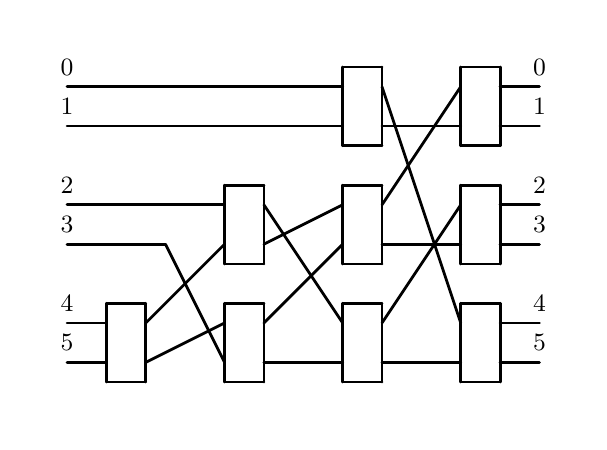
\begin{tikzpicture}[line cap=round,line join=round,>=triangle 45,x=0.5cm,y=0.5cm]

\clip(-2.,-1.) rectangle (12.,9.);

\draw (-1.,8.) node {\small 0};
\draw (-1.,7.) node {\small 1};
\draw (-1.,5.) node {\small 2};
\draw (-1.,4.) node {\small 3};
\draw (-1.,2.) node {\small 4};
\draw (-1.,1.) node {\small 5};

\draw (11.,8.) node {\small 0};
\draw (11.,7.) node {\small 1};
\draw (11.,5.) node {\small 2};
\draw (11.,4.) node {\small 3};
\draw (11.,2.) node {\small 4};
\draw (11.,1.) node {\small 5};

\draw [line width=1.pt] (0.,0.)-- (1.,0.);
\draw [line width=1.pt] (1.,0.)-- (1.,2.);
\draw [line width=1.pt] (1.,2.)-- (0.,2.);
\draw [line width=1.pt] (0.,0.)-- (0.,2.);
\draw [line width=1.pt] (3.,2.)-- (3.,0.);
\draw [line width=1.pt] (4.,0.)-- (3.,0.);
\draw [line width=1.pt] (4.,0.)-- (4.,2.);
\draw [line width=1.pt] (4.,2.)-- (3.,2.);
\draw [line width=1.pt] (6.,2.)-- (6.,0.);
\draw [line width=1.pt] (6.,0.)-- (7.,0.);
\draw [line width=1.pt] (7.,0.)-- (7.,2.);
\draw [line width=1.pt] (7.,2.)-- (6.,2.);
\draw [line width=1.pt] (9.,2.)-- (9.,0.);
\draw [line width=1.pt] (9.,0.)-- (10.,0.);
\draw [line width=1.pt] (10.,0.)-- (10.,2.);
\draw [line width=1.pt] (10.,2.)-- (9.,2.);
\draw [line width=1.pt] (6.,3.)-- (7.,3.);
\draw [line width=1.pt] (7.,3.)-- (7.,5.);
\draw [line width=1.pt] (7.,5.)-- (6.,5.);
\draw [line width=1.pt] (6.,5.)-- (6.,3.);
\draw [line width=1.pt] (9.,3.)-- (10.,3.);
\draw [line width=1.pt] (10.,3.)-- (10.,5.);
\draw [line width=1.pt] (10.,5.)-- (9.,5.);
\draw [line width=1.pt] (9.,5.)-- (9.,3.);
\draw [line width=1.pt] (9.,6.)-- (10.,6.);
\draw [line width=1.pt] (10.,6.)-- (10.,8.);
\draw [line width=1.pt] (10.,8.)-- (9.,8.);
\draw [line width=1.pt] (9.,6.)-- (9.,8.);
\draw [line width=1.pt] (3.,5.)-- (3.,3.);
\draw [line width=1.pt] (4.,3.)-- (3.,3.);
\draw [line width=1.pt] (4.,3.)-- (4.,5.);
\draw [line width=1.pt] (4.,5.)-- (3.,5.);
\draw [line width=1.pt] (6.,6.)-- (7.,6.);
\draw [line width=1.pt] (7.,6.)-- (7.,8.);
\draw [line width=1.pt] (7.,8.)-- (6.,8.);
\draw [line width=1.pt] (6.,8.)-- (6.,6.);
\draw [line width=1.pt] (1.,1.5)-- (3.,3.5);
\draw [line width=1.pt] (3.,4.5)-- (-1.,4.5);
\draw [line width=1.pt] (0.,0.5)-- (-1.,0.5);
\draw [line width=1.pt] (0.,1.5)-- (-1.,1.5);
\draw [line width=1.pt] (1.,0.5)-- (3.,1.5);
\draw [line width=1.pt] (-1.,3.5)-- (1.5,3.5);
\draw [line width=1.pt] (1.5,3.5)-- (3.,0.5);
\draw [line width=1.pt] (6.,6.5)-- (-1.,6.5);
\draw [line width=1.pt] (6.,7.5)-- (-1.,7.5);
\draw [line width=1.pt] (4.,4.5)-- (6.,1.5);
\draw [line width=1.pt] (4.,3.5)-- (6.,4.5);
\draw [line width=1.pt] (4.,1.5)-- (6.,3.5);
\draw [line width=1.pt] (4.,0.5)-- (6.,0.5);
\draw [line width=1.pt] (7.,7.5)-- (9.,1.5);
\draw [line width=1.pt] (7.,6.5)-- (9.,6.5);
\draw [line width=1.pt] (7.,4.5)-- (9.,7.5);
\draw [line width=1.pt] (7.,3.5)-- (9.,3.5);
\draw [line width=1.pt] (7.,1.5)-- (9.,4.5);
\draw [line width=1.pt] (7.,0.5)-- (9.,0.5);
\draw [line width=1.pt] (10.,1.5)-- (11.,1.5);
\draw [line width=1.pt] (10.,0.5)-- (11.,0.5);
\draw [line width=1.pt] (10.,3.5)-- (11.,3.5);
\draw [line width=1.pt] (10.,4.5)-- (11.,4.5);
\draw [line width=1.pt] (10.,6.5)-- (11.,6.5);
\draw [line width=1.pt] (10.,7.5)-- (11.,7.5);
\end{tikzpicture}
\end{center}

\subsection{Najprostsze sieci}

Zastanówmy się najpierw, czy istnieje sieć o 6 wejściach i 6 wyjściach mająca rozmiar równy 9, która realizuje wszystkie permutacje z \(S_6\)?

\vspace{1em}

Odpowiedź to nie -- łatwo zauważyć, że każdy przełącznik zwiększa liczbę permutacji realizowanych przez sieć co najwyżej dwukrotnie. Wobec tego taka sieć realizuje co najwyżej \(2^9 = 512\) permutacji. Zarazem \(6! = 720 > 512\),  czyli taka sieć nie może istnieć. 

\vspace{1em}

Jakie sieci zatem istnieją? W poniższych rozważaniach pochylimy się nad sieciami głębokości co najwyżej 2 realizującymi identyczność i pewną inną permutację. Konstrukcje tych sieci przeprowadzamy tak, jak autorzy pracy \cite{klo}. Będą one pomocne przy tworzeniu sieci realizującej przesunięcia cykliczne o potęgi 2. 

\begin{lem}\label{lem:perm_symetrie}
    Dla dowolnego \(n\) oraz \(k \in \{0, 1, \ldots, n-1\}\) istnieje sieć o \(n\) wejściach i \(n\) wyjściach o głębokości 1 i rozmiarze co najwyżej \(\floor{\frac n 2}\) realizująca \(\id{n}\) i \(\sym{n}{k}\).
\end{lem}

\begin{proof}
    Ustalmy \(n\) oraz \(k \in \{0, 1, \ldots, n-1\}\). Zauważmy, że 
    \[
    \sym{n}{k} \circ \sym{n}{k} = \id{n} \td
    \]
    Wobec tego permutacja \(\sym n k\) jest inwolucją, a co za tym idzie -- składa się z cykli o rozmiarze co najwyżej 2. Konstrukcja sieci wygląda następująco:
    \begin{itemize}
        \item każdemu cyklowi postaci \((i,j)\) przypisujemy przełącznik, który na wejściach przyjmuje sygnały \(i\) oraz \(j\) z wejścia sieci, a przewody na jego wyjściach prowadzą do wyjść sieci o numerach \(i\) oraz \(j\),
        \item każdemu cyklowi jednoelementowemu postaci \((i)\) przypisujemy przewód biegnący od \(i\)--tego wejścia do \(i\)--tego wyjścia sieci.
    \end{itemize}
    Oczywiście w ten sposób używamy co najwyżej \(\floor{\frac{n}{2}}\) przełączników. 
    Ponadto jeśli wszystkie przełączniki są w stanie nieaktywnym, sieć realizuje \(\id n\), natomiast jeśli wszystkie są w stanie aktywnym, to realizuje \(\sym n k\).
\end{proof}


\begin{center}
    
\todo{Poprawić rysunek -- sym \(n=4\), \(k=2\)}

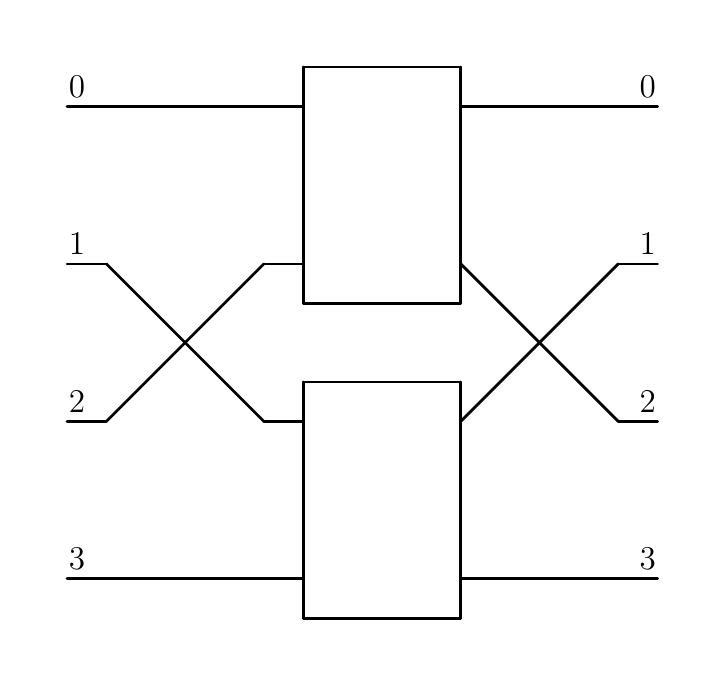
\begin{tikzpicture}[line cap=round,line join=round,>=triangle 45,x=0.5cm,y=0.5cm]
\clip(-7.,-1.) rectangle (10.,15.);
\draw [line width=1.pt] (0.,0.)-- (4.,0.);
\draw [line width=1.pt] (4.,0.)-- (4.,6.);
\draw [line width=1.pt] (4.,6.)-- (0.,6.);
\draw [line width=1.pt] (0.,6.)-- (0.,0.);
\draw [line width=1.pt] (0.,8.)-- (4.,8.);
\draw [line width=1.pt] (4.,8.)-- (4.,14.);
\draw [line width=1.pt] (4.,14.)-- (0.,14.);
\draw [line width=1.pt] (0.,14.)-- (0.,8.);
\draw [line width=1.pt] (0.,13.)-- (-1.,13.);
\draw [line width=1.pt] (0.,9.)-- (-1.,9.);
\draw [line width=1.pt] (0.,5.)-- (-1.,5.);
\draw [line width=1.pt] (0.,1.)-- (-1.,1.);
\draw [line width=1.pt] (-6.,9.)-- (-5.,9.);
\draw [line width=1.pt] (-5.,9.)-- (-1.,5.);
\draw [line width=1.pt] (-5.,5.)-- (-1.,9.);
\draw [line width=1.pt] (4.,13.)-- (9.,13.);
\draw [line width=1.pt] (4.,9.)-- (8.,5.);
\draw [line width=1.pt] (8.,5.)-- (9.,5.);
\draw [line width=1.pt] (4.,5.)-- (8.,9.);
\draw [line width=1.pt] (8.,9.)-- (9.,9.);
\draw [line width=1.pt] (4.,1.)-- (9.,1.);
\draw [line width=1.pt] (-6.,13.)-- (-5.,13.);
\draw [line width=1.pt] (-5.,13.)-- (-1.,13.);
\draw [line width=1.pt] (-6.,5.)-- (-5.,5.);
\draw [line width=1.pt] (-6.,1.)-- (-5.,1.);
\draw [line width=1.pt] (-5.,1.)-- (-1.,1.);

\draw (-5.75,13.5) node {\large 0};
\draw (-5.75,9.5) node {\large 1};
\draw (-5.75,5.5) node {\large 2};
\draw (-5.75,1.5) node {\large 3};

\draw (8.75,13.5) node {\large 0};
\draw (8.75,9.5) node {\large 1};
\draw (8.75,5.5) node {\large 2};
\draw (8.75,1.5) node {\large 3};

% \begin{scriptsize}
% \draw[color=black] (-5.5,12.5) node {\large 0 \par};
% \draw[color=black] (-5.5,8.5) node {\large 1 \par};
% \draw[color=black] (-5.5,4.5) node {\large 2 \par};
% \draw[color=black] (-5.5,0) node {\large 3 \par};
% \end{scriptsize}
\end{tikzpicture}

{\it  Konstrukcja z lematu \ref{lem:perm_symetrie} dla \(n=4\) i \(k=2\)}
\end{center}

Lemat \ref{lem:perm_symetrie} można jednak uogólnić -- zauważmy, że nie korzystamy z żadnych własności symetrii, poza tym, że \( \sym n k \circ \sym n k = \id n \).

\begin{lem}\label{lem:perm_inwolucje}
    Dla dowolnego \(n\) oraz \(\sigma \in S_n\), które jest inwolucją (to znaczy \(\sigma \circ \sigma = \id n\)) istnieje sieć o \(n\) wejściach i \(n\) wyjściach o głębokości 1 i rozmiarze co najwyżej \(\floor{\frac{n}{2}}\) realizująca \(\id n\) oraz \(\sigma\).
\end{lem}

\begin{proof}
    Konstrukcja jest identyczna jak ta w lemacie \ref{lem:perm_symetrie}.
\end{proof}

\begin{lem}\label{lem:perm_shifty}
     Dla dowolnego \(n\) oraz \(k \in \{0, 1, \ldots, n-1\}\) istnieje sieć o \(n\) wejściach i \(n\) wyjściach o głębokości 2 realizująca \(\id n\) i \(\shift{n}{k}\).
\end{lem}

\begin{proof}
    Ustalmy \(n\). Zauważmy, że
    \[
    \sym n k (\sym n 0 (i)) = \sym n k (-i \mod n) = (k - (-i)) \mod n = (k + i) \mod n  = \shift n k (i)
    \]
    dla każdego \(i \in \{0, 1, \ldots, n-1\}\). Wobec tego \(\shift n k = \sym n k \circ \sym n 0\). Stwórzmy zatem sieć przełączników o dwóch warstwach -- pierwsza z nich niech będzie siecią realizującą \(\id n\) i \(\sym n 0\), a druga siecią realizującą \(\id n\) i  \(\sym n k\) (jak w lemacie \ref{lem:perm_symetrie}). Taka sieć ma głębokość 2. Jeśli wszystkie przełączniki są nieaktywne, to realizuje \(\id n\), natomiast jeśli wszystkie są aktywne, to z powyższego rachunku wynika, że realizuje \(\shift n k\).
\end{proof}

\todo{Poprawić rysunek -- shift \(n=4\), \(k=2\)}

\begin{center}
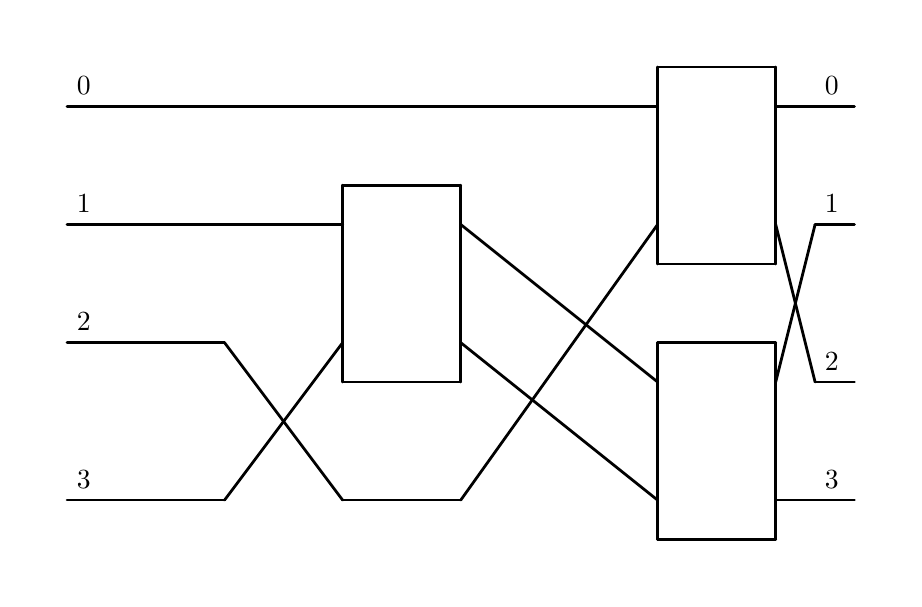
\begin{tikzpicture}[line cap=round,line join=round,>=triangle 45,x=0.5cm,y=0.5cm]
\clip(-1.,-1.) rectangle (21.,13.);
\draw [line width=1.pt] (0.,1.)-- (4.,1.);
\draw [line width=1.pt] (0.,5.)-- (4.,5.);
\draw [line width=1.pt] (0.,8.)-- (4.,8.);
\draw [line width=1.pt] (7.,9.)-- (10.,9.);
\draw [line width=1.pt] (10.,9.)-- (10.,4.);
\draw [line width=1.pt] (10.,4.)-- (7.,4.);
\draw [line width=1.pt] (7.,4.)-- (7.,9.);
\draw [line width=1.pt] (4.,1.)-- (7.,5.);
\draw [line width=1.pt] (4.,8.)-- (7.,8.);
\draw [line width=1.pt] (4.,5.)-- (7.,1.);
\draw [line width=1.pt] (7.,1.)-- (10.,1.);
\draw [line width=1.pt] (10.,1.)-- (15.,8.);
\draw [line width=1.pt] (10.,5.)-- (15.,1.);
\draw [line width=1.pt] (10.,8.)-- (15.,4.);
\draw [line width=1.pt] (15.,12.)-- (15.,7.);
\draw [line width=1.pt] (15.,7.)-- (18.,7.);
\draw [line width=1.pt] (18.,7.)-- (18.,12.);
\draw [line width=1.pt] (18.,12.)-- (15.,12.);
\draw [line width=1.pt] (15.,5.)-- (18.,5.);
\draw [line width=1.pt] (18.,5.)-- (18.,0.);
\draw [line width=1.pt] (18.,0.)-- (15.,0.);
\draw [line width=1.pt] (15.,0.)-- (15.,5.);
\draw [line width=1.pt] (0.,11.)-- (15.,11.);
\draw [line width=1.pt] (18.,11.)-- (20.,11.);
\draw [line width=1.pt] (18.,8.)-- (19.,4.);
\draw [line width=1.pt] (18.,4.)-- (19.,8.);
\draw [line width=1.pt] (18.,1.)-- (20.,1.);
\draw [line width=1.pt] (19.,8.)-- (20.,8.);
\draw [line width=1.pt] (19.,4.)-- (20.,4.);
\draw (0,12) node[anchor=north west] {0};
\draw (0,9) node[anchor=north west] {1};
\draw (0,6) node[anchor=north west] {2};
\draw (0,2) node[anchor=north west] {3};
\draw (19,12) node[anchor=north west] {0};
\draw (19,9) node[anchor=north west] {1};
\draw (19,5) node[anchor=north west] {2};
\draw (19,2) node[anchor=north west] {3};
\end{tikzpicture}

{\it Konstrukcja z lematu \ref{lem:perm_shifty} dla \(n=4\) i \(k=2\)}
\end{center}

\begin{lem}
    Dla dowolnego \(n\) oraz \(\sigma \in S_n\) istnieje sieć o  \(n\) wejściach i \(n\) wyjściach o głębokości 2 realizująca \(\id n\) i \(\sigma\).
\end{lem}

\begin{proof}
    Ustalmy \(n\) oraz \(\sigma \in S_n\). Oczywiście \(\sigma\) może być przedstawiona jako złożenie cykli rozłącznych:
    \[
        \sigma = \sigma_1 \circ \sigma_2 \circ \ldots \circ \sigma_k \td
    \]
    Prostą konsekwencją lematu \ref{lem:perm_shifty} jest to, że istnieje sieć o głębokości 2, która realizuje \(\id n\) oraz \(\sigma_i\) dla każdego \(i\). Konstrukcja żądanej sieci polega na złożeniu tych sieci dla każdego \(\sigma_i\). Z rozłączności cykli wynika, że będzie miała ona głębokość równą 2. 
\end{proof}



% ---------- sieć Beneša-Waksmana -----------------

\section{Sieć Beneša--Waksmana}

W tym rozdziale będziemy zajmować się siecią, która realizuje wszystkie możliwe permutacje dla ustalonego \(n\). Dla uproszczenia przyjmiemy, że $n = 2^k$ dla pewnego \(k \in \N\).
%\begin{pyt}
%    Czy istnieje sieć realizująca wszystkie permutacje z \(S_n\)?
%\end{pyt}
%Odpowiedź to tak. 
%\todo{Przykład jak konstruować nie optymalnie sieci permutacji}

% \vspace{.5em}

\subsection{Ograniczenie dolne}

Najpierw zastanówmy się nad ograniczeniem dolnym -- czy istnieje asymptotyczne oszacowanie minimalnej liczby przełączników potrzebnych do zrealizowania wszystkich permutacji z \(S_n\)?
 
% \begin{pyt}
%     Jaka jest minimalna liczba przełączników, potrzebnych żeby zrealizować wszystkie permutacje z \(S_n\)?
% \end{pyt}
\begin{tw}
    Dowolna sieć, która realizuje wszystkie permutacje z \(S_n\), ma  \(\Omega(n \log n )\) przełączników.
\end{tw}
\begin{proof}
Ustalmy $n \in \mathbb{N}$ i sieć realizującą wszystkie permutacje z \(S_n\). Oznaczmy liczbę przełączników w tej sieci przez \(p\).
Zauważmy, że każdy przełącznik, zwiększa liczbę realizowanych permutacji co najwyżej dwukrotnie.
Wobec tego $log(n!) \leq p$. Ze wzoru Stirlinga z możemy oszacować \(n!\) z dołu przez $(n/e)^n$. Otrzymujemy zatem
\[
    \log (n!) \geq \log ( (n/e)^n ) = n(\log n - \log e) = \Omega(n \log n)
\]
\end{proof}

\subsection{Konstrukcja i dowód poprawności}

Konstrukcja polega na podzieleniu problemu na dwa identyczne podproblemy i pomysłowym połączeniu odpowiadających im podsieci w pełne rozwiązanie.

\vspace{.5em}

Ustalmy \(n\). Rekurencyjne konstruujemy dwie identyczne sieci realizujące wszystkie permutacje z \(S_{n/2}\). Jedną z nich nazwijmy \emph{białą}, a drugą \emph{czarną}. 

\vspace{.5em}

Tworzymy warstwę wejściową przewodników. Przewody z \(n\) wejść sieci kierujemy do \(n/2\) przewodników w taki sposób, że do \(k\)--tego przełącznika trafiają przewody z wyjść \(2k\) (na wejście 0) oraz \(2k+1\) (na wejście 1) dla \(k = 0, 1, \ldots, n/2 - 1\). Natomiast z przewody z wyjścia 0 i 1 \(k\)--tego przewodnika kierujemy do \(k\)--tego wejścia odpowiednio białej i czarnej podsieci. 

\vspace{.5em}

Analogicznie tworzymy warstwę wyjściową przełączników. Dokładniej kładziemy \(n/2\) przełączników tak, że przewody z wyjścia 0 i 1 \(k\)--tego przewodnika prowadzą odpowiednio do wyjść sieci o numerach \(2k\) i \(2k+1\). Natomiast do wejść 0 i 1 \(k\)--tego przewodnika prowadzimy przewód z \(k\)--tego wyjścia odpowiednio białej i czarnej podsieci. 

\vspace{.5em}

Konstrukcję schematycznie przedstawiono na poniższym rysunku.

\begin{center}
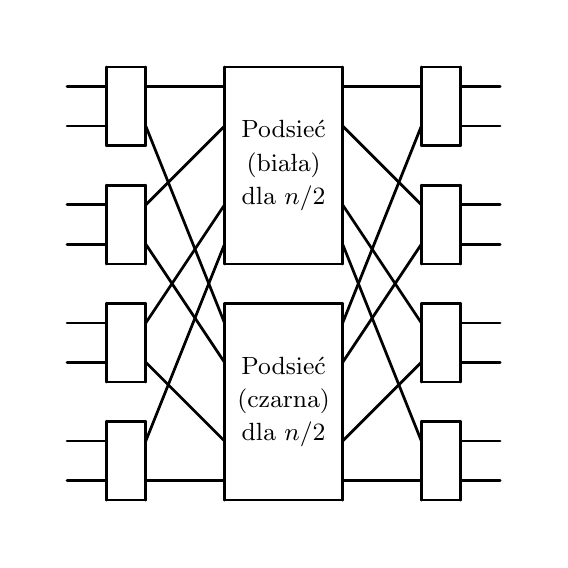
\begin{tikzpicture}[line cap=round,line join=round,>=triangle 45,x=0.5cm,y=0.5cm]
\clip(-2.,-1.) rectangle (11.,12.);
\draw [line width=1.pt] (0.,0.)-- (1.,0.);
\draw [line width=1.pt] (1.,0.)-- (1.,2.);
\draw [line width=1.pt] (1.,2.)-- (0.,2.);
\draw [line width=1.pt] (0.,2.)-- (0.,0.);
\draw [line width=1.pt] (0.,3.)-- (1.,3.);
\draw [line width=1.pt] (1.,3.)-- (1.,5.);
\draw [line width=1.pt] (1.,5.)-- (0.,5.);
\draw [line width=1.pt] (0.,5.)-- (0.,3.);
\draw [line width=1.pt] (0.,6.)-- (1.,6.);
\draw [line width=1.pt] (1.,6.)-- (1.,8.);
\draw [line width=1.pt] (1.,8.)-- (0.,8.);
\draw [line width=1.pt] (0.,8.)-- (0.,6.);
\draw [line width=1.pt] (0.,9.)-- (1.,9.);
\draw [line width=1.pt] (1.,9.)-- (1.,11.);
\draw [line width=1.pt] (1.,11.)-- (0.,11.);
\draw [line width=1.pt] (0.,11.)-- (0.,9.);
\draw [line width=1.pt] (3.,11.)-- (3.,6.);
\draw [line width=1.pt] (3.,6.)-- (6.,6.);
\draw [line width=1.pt] (6.,11.)-- (6.,6.);
\draw [line width=1.pt] (6.,11.)-- (3.,11.);
\draw [line width=1.pt] (3.,5.)-- (3.,0.);
\draw [line width=1.pt] (3.,5.)-- (6.,5.);
\draw [line width=1.pt] (6.,5.)-- (6.,0.);
\draw [line width=1.pt] (6.,0.)-- (3.,0.);
\draw [line width=1.pt] (8.,11.)-- (9.,11.);
\draw [line width=1.pt] (9.,11.)-- (9.,9.);
\draw [line width=1.pt] (9.,9.)-- (8.,9.);
\draw [line width=1.pt] (8.,9.)-- (8.,11.);
\draw [line width=1.pt] (8.,8.)-- (8.,6.);
\draw [line width=1.pt] (8.,6.)-- (9.,6.);
\draw [line width=1.pt] (9.,6.)-- (9.,8.);
\draw [line width=1.pt] (9.,8.)-- (8.,8.);
\draw [line width=1.pt] (8.,5.)-- (8.,3.);
\draw [line width=1.pt] (8.,3.)-- (9.,3.);
\draw [line width=1.pt] (9.,3.)-- (9.,5.);
\draw [line width=1.pt] (9.,5.)-- (8.,5.);
\draw [line width=1.pt] (8.,2.)-- (8.,0.);
\draw [line width=1.pt] (8.,0.)-- (9.,0.);
\draw [line width=1.pt] (9.,0.)-- (9.,2.);
\draw [line width=1.pt] (9.,2.)-- (8.,2.);
\draw [line width=1.pt] (0.,10.5)-- (-1.,10.5);
\draw [line width=1.pt] (0.,9.5)-- (-1.,9.5);
\draw [line width=1.pt] (0.,7.5)-- (-1.,7.5);
\draw [line width=1.pt] (0.,6.5)-- (-1.,6.5);
\draw [line width=1.pt] (0.,4.5)-- (-1.,4.5);
\draw [line width=1.pt] (0.,3.5)-- (-1.,3.5);
\draw [line width=1.pt] (0.,1.5)-- (-1.,1.5);
\draw [line width=1.pt] (0.,0.5)-- (-1.,0.5);
\draw [line width=1.pt] (1.,10.5)-- (3.,10.5);
\draw [line width=1.pt] (1.,9.5)-- (3.,4.5);
\draw [line width=1.pt] (1.,7.5)-- (3.,9.5);
\draw [line width=1.pt] (1.,6.5)-- (3.,3.5);
\draw [line width=1.pt] (1.,4.5)-- (3.,7.5);
\draw [line width=1.pt] (1.,3.5)-- (3.,1.5);
\draw [line width=1.pt] (1.,1.5)-- (3.,6.5);
\draw [line width=1.pt] (1.,0.5)-- (3.,0.5);
\draw [line width=1.pt] (6.,10.5)-- (8.,10.5);
\draw [line width=1.pt] (8.,9.5)-- (6.,4.5);
\draw [line width=1.pt] (8.,7.5)-- (6.,9.5);
\draw [line width=1.pt] (8.,6.5)-- (6.,3.5);
\draw [line width=1.pt] (8.,4.5)-- (6.,7.5);
\draw [line width=1.pt] (8.,3.5)-- (6.,1.5);
\draw [line width=1.pt] (8.,1.5)-- (6.,6.5);
\draw [line width=1.pt] (8.,0.5)-- (6.,0.5);
\draw [line width=1.pt] (9.,10.5)-- (10.,10.5);
\draw [line width=1.pt] (9.,9.5)-- (10.,9.5);
\draw [line width=1.pt] (9.,7.5)-- (10.,7.5);
\draw [line width=1.pt] (9.,6.5)-- (10.,6.5);
\draw [line width=1.pt] (9.,4.5)-- (10.,4.5);
\draw [line width=1.pt] (9.,3.5)-- (10.,3.5);
\draw [line width=1.pt] (9.,1.5)-- (10.,1.5);
\draw [line width=1.pt] (9.,0.5)-- (10.,0.5);

\draw (4.5,8.5) node[align=center] {\small Podsieć \\ \small (biała) \\ \small dla \(n/2\)};
\draw (4.5,2.5) node[align=center] {\small Podsieć \\ \small (czarna) \\ \small dla \(n/2\)};
\end{tikzpicture}
\end{center}


\begin{tw}
    Sieć Beneša--Waksmana realizuje wszystkie permutacje.
\end{tw}

\begin{proof}
Przeprowadzimy dowód przez indukcję, korzystając z rekurencyjnej struktury sieci. 

    \begin{enumerate} 
        \item Podstawa indukcji dla $n = 1$ oraz $n = 2$. \\
        Dla $n = 1$ sieć Beneša--Waksmana jest prostu przewodem. Z kolei dla $n = 2$ jest to pojedynczy przełącznik.

        \item Krok indukcyjny. Weźmy dowolne $n = 2^k$ dla pewnego $k$ naturalnego i załóżmy, że sieć dla \(n/2\) konstruowana w sposób opisany powyżej realizuje wszystkie permutacje $n/2$--elementowe. 
        Ustalmy \(\pi \in S_n\).
        
        Zauważmy, że wystarczy wskazać podział zbioru \(\{0, 1, \ldots, n-1\}\) na dwa podzbiory \(n/2\)--elementowe (nazwijmy je \emph{białym} i \emph{czarnym}) o następującej własności: dla dowolnego \(k = 0, 1, \ldots, n/2 - 1\) liczby \(2k\) i \(2k+1\) należą do różnych zbiorów podziału oraz analogicznie liczby \(\pi(2k)\) i \(\pi(2k+1)\) należą do różnych zbiorów podziału.

        \vspace{.5em}

        Istotnie -- zakładając, że istnieje taki podział, ustawienie przełączników realizujące \(\pi\) wygląda następująco: 

        \begin{itemize}
            \item jeśli \(2k\) jest w białym zbiorze, a \(2k+1\) w czarnym, to \(k\)--temu przełącznikowi z warstwy wejściowej nadajemy stan nieaktywny,
            \item w przeciwnym przypadku \(k\)--temu przełącznikowi z warstwy wyjściowej nadajemy stan aktywny.  
        \end{itemize}
        dla \(k = 0, 1, \ldots, n/2-1\). Analogicznie nadajemy stan \(k\)--temu przełącznikowi na wyjściu:
        \begin{itemize}
            \item jeśli \(\pi(2k)\) jest w białym zbiorze, a \(\pi(2k+1)\) w czarnym, to \(k\)--temu przełącznikowi nadajemy stan nieaktywny,
            \item w przeciwnym przypadku \(k\)--temu przełącznikowi nadajemy stan aktywny.  
        \end{itemize}

        Natomiast o właściwe ustawienie liczb wewnątrz \emph{białego} i \emph{czarnego} zbioru ,,zadbają'' rekurencyjnie skonstruowane sieci.

        \vspace{.1em}

        Stwórzmy zatem podział spełniający powyższe warunki. 

        \vspace{.1em}
        
        % Niech $V = V_i \cup V_m $ będzie zbiorem wierzchołków.
        Niech \(V_i = \{ 0, 1, \ldots, n-1 \}\) będzie zbiorem wierzchołków odpowiadających portom wejściowym sieci (\(j\)--ty port wejściowy  utożsamiamy z wierzchołkiem \(j\)). Łączymy ze sobą wierzchołki, które odpowiadają wejściom tego samego przełącznika z warstwy wejściowej. Dokładniej łączymy krawędzią  wierzchołki $0$ i $1$, $2$ i $3$, ... , $n-2$ i $n-1$. 

        \vspace{.1em}
        Niech $V_o = \{0', 1', \ldots, (n-1)'\}$ będzie zbiorem wierzchołków, które odpowiadają portom wyjściowym sieci (\(j\)--ty port wyjściowy utożsamiamy z \(k'\), takim że \(\pi(j) = k\)). Łączymy krawędzią te, które są ze sobą w jednym przełączniku w warstwie wyjściowej (czyli \(\pi(2j)'\) oraz \(\pi(2j+1)'\) dla \(j = 0, 1, \ldots, n/2 - 1\)). 

        
        Ponadto łączymy krawędzią wierzchołki o etykietach $j$ oraz $j'$.

        Poniżej przedstawiamy schematyczny graf dla \(n = 8\) oraz 
        \[
            \pi = \begin{pmatrix}
                0 & 1 & 2 & 3 & 4 & 5 & 6 & 7 \\
                3 & 7 & 0 & 1 & 4 & 5 & 2 & 6
              \end{pmatrix}.
        \]

\begin{center}
        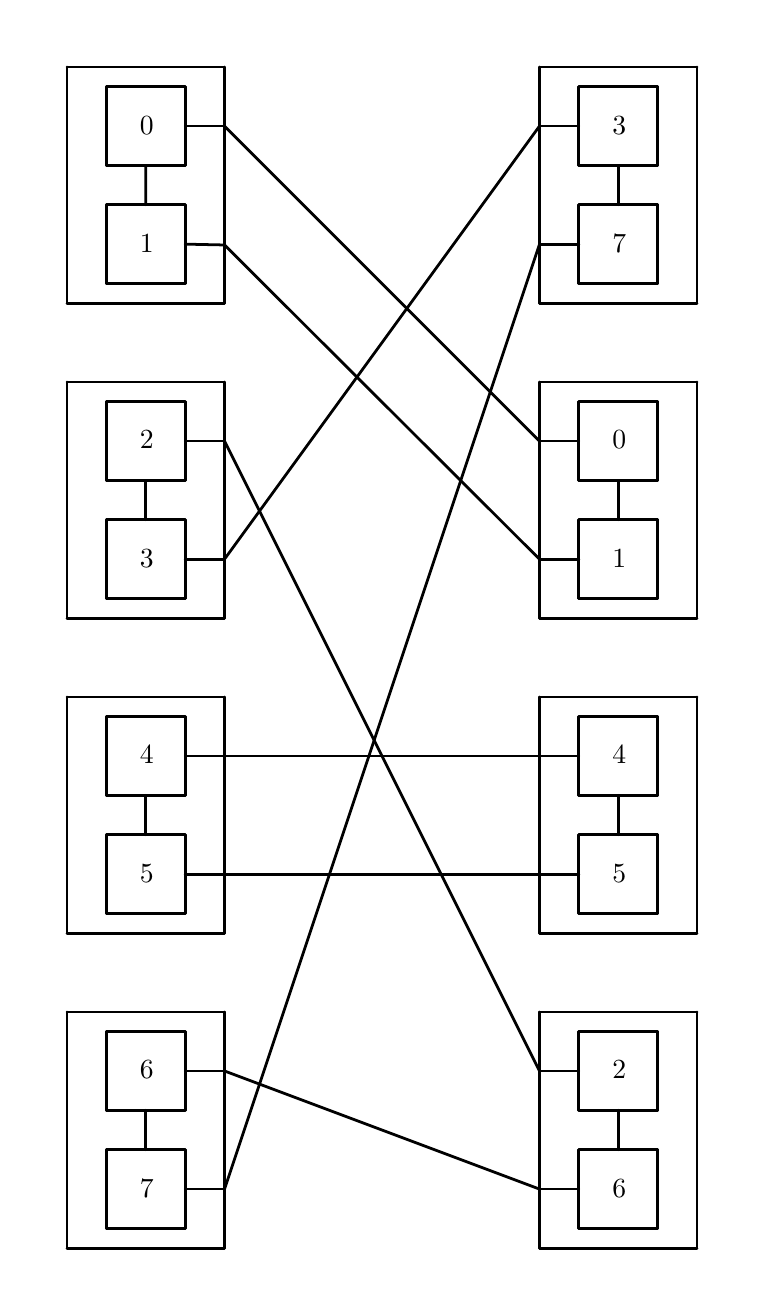
\begin{tikzpicture}[line cap=round,line join=round,>=triangle 45,x=0.5cm,y=0.5cm]
\clip(-1.,-1.) rectangle (17.,31.);
\draw [line width=1.pt] (0.,0.)-- (4.,0.);
\draw [line width=1.pt] (4.,0.)-- (4.,6.);
\draw [line width=1.pt] (4.,6.)-- (0.,6.);
\draw [line width=1.pt] (0.,6.)-- (0.,0.);
\draw [line width=1.pt] (0.,8.)-- (4.,8.);
\draw [line width=1.pt] (4.,8.)-- (4.,14.);
\draw [line width=1.pt] (4.,14.)-- (0.,14.);
\draw [line width=1.pt] (0.,14.)-- (0.,8.);
\draw [line width=1.pt] (0.,16.)-- (4.,16.);
\draw [line width=1.pt] (4.,16.)-- (4.,22.);
\draw [line width=1.pt] (4.,22.)-- (0.,22.);
\draw [line width=1.pt] (0.,22.)-- (0.,16.);
\draw [line width=1.pt] (0.,24.)-- (4.,24.);
\draw [line width=1.pt] (4.,24.)-- (4.,30.);
\draw [line width=1.pt] (4.,30.)-- (0.,30.);
\draw [line width=1.pt] (0.,30.)-- (0.,24.);
\draw [line width=1.pt] (12.,30.)-- (16.,30.);
\draw [line width=1.pt] (16.,30.)-- (16.,24.);
\draw [line width=1.pt] (16.,24.)-- (12.,24.);
\draw [line width=1.pt] (12.,24.)-- (12.,30.);
\draw [line width=1.pt] (12.,22.)-- (16.,22.);
\draw [line width=1.pt] (16.,22.)-- (16.,16.);
\draw [line width=1.pt] (16.,16.)-- (12.,16.);
\draw [line width=1.pt] (12.,16.)-- (12.,22.);
\draw [line width=1.pt] (12.,14.)-- (16.,14.);
\draw [line width=1.pt] (16.,14.)-- (16.,8.);
\draw [line width=1.pt] (16.,8.)-- (12.,8.);
\draw [line width=1.pt] (12.,8.)-- (12.,14.);
\draw [line width=1.pt] (12.,6.)-- (16.,6.);
\draw [line width=1.pt] (16.,6.)-- (16.,0.);
\draw [line width=1.pt] (16.,0.)-- (12.,0.);
\draw [line width=1.pt] (12.,0.)-- (12.,6.);
\draw [line width=1.pt] (4.,28.5)-- (12.,20.5);
\draw [line width=1.pt] (4.,25.480146267130415)-- (12.,17.5);
\draw [line width=1.pt] (4.,17.5)-- (12.,28.5);
\draw [line width=1.pt] (12.,25.5)-- (4.,1.5);
\draw [line width=1.pt] (4.,4.5)-- (12.,1.5);
\draw [line width=1.pt] (12.,4.5)-- (4.,20.5);
\draw [line width=1.pt] (4.,12.5)-- (12.,12.5);
\draw [line width=1.pt] (4.,9.5)-- (12.,9.5);
\draw [line width=1.pt] (1.,29.5)-- (1.,27.5);
\draw [line width=1.pt] (1.,27.5)-- (3.,27.5);
\draw [line width=1.pt] (3.,27.5)-- (3.,29.5);
\draw [line width=1.pt] (3.,29.5)-- (1.,29.5);
\draw [line width=1.pt] (1.,26.5)-- (3.,26.5);
\draw [line width=1.pt] (3.,24.5)-- (3.,26.5);
\draw [line width=1.pt] (3.,24.5)-- (1.,24.5);
\draw [line width=1.pt] (1.,24.5)-- (1.,26.5);
\draw [line width=1.pt] (4.,28.5)-- (3.,28.5);
\draw [line width=1.pt] (3.,25.501229087688593)-- (4.,25.480146267130415);
\draw [line width=1.pt] (2.,27.5)-- (1.9995868314540757,26.5);
\draw [line width=1.pt] (13.,16.5)-- (15.,16.5);
\draw [line width=1.pt] (15.,16.5)-- (15.,18.5);
\draw [line width=1.pt] (15.,18.5)-- (13.,18.5);
\draw [line width=1.pt] (13.,18.5)-- (13.,16.5);
\draw [line width=1.pt] (13.,21.5)-- (13.,19.5);
\draw [line width=1.pt] (13.,19.5)-- (15.,19.5);
\draw [line width=1.pt] (15.,19.5)-- (15.,21.5);
\draw [line width=1.pt] (15.,21.5)-- (13.,21.5);
\draw [line width=1.pt] (14.,19.5)-- (14.,18.5);
\draw [line width=1.pt] (12.,20.5)-- (13.,20.5);
\draw [line width=1.pt] (13.,17.5)-- (12.,17.5);
\draw [line width=1.pt] (13.,29.5)-- (15.,29.5);
\draw [line width=1.pt] (15.,29.5)-- (15.,27.5);
\draw [line width=1.pt] (15.,27.5)-- (13.,27.5);
\draw [line width=1.pt] (13.,27.5)-- (13.,29.5);
\draw [line width=1.pt] (13.,26.5)-- (15.,26.5);
\draw [line width=1.pt] (15.,26.5)-- (15.,24.5);
\draw [line width=1.pt] (15.,24.5)-- (13.,24.5);
\draw [line width=1.pt] (13.,24.5)-- (13.,26.5);
\draw [line width=1.pt] (12.,28.5)-- (13.,28.5);
\draw [line width=1.pt] (14.,27.5)-- (14.,26.5);
\draw [line width=1.pt] (13.,25.5)-- (12.,25.5);
\draw [line width=1.pt] (1.,21.5)-- (3.,21.5);
\draw [line width=1.pt] (3.,21.5)-- (3.,19.5);
\draw [line width=1.pt] (3.,19.5)-- (1.,19.5);
\draw [line width=1.pt] (1.,19.5)-- (1.,21.5);
\draw [line width=1.pt] (1.,16.5)-- (3.,16.5);
\draw [line width=1.pt] (3.,16.5)-- (3.,18.5);
\draw [line width=1.pt] (3.,18.5)-- (1.,18.5);
\draw [line width=1.pt] (1.,18.5)-- (1.,16.5);
\draw [line width=1.pt] (4.,17.5)-- (3.,17.5);
\draw [line width=1.pt] (2.,18.5)-- (2.,19.5);
\draw [line width=1.pt] (3.,20.5)-- (4.,20.5);
\draw [line width=1.pt] (13.,5.5)-- (15.,5.5);
\draw [line width=1.pt] (15.,5.5)-- (15.,3.5);
\draw [line width=1.pt] (15.,3.5)-- (13.,3.5);
\draw [line width=1.pt] (13.,3.5)-- (13.,5.5);
\draw [line width=1.pt] (12.,4.5)-- (13.,4.5);
\draw [line width=1.pt] (13.,2.5)-- (15.,2.5);
\draw [line width=1.pt] (15.,2.5)-- (15.,0.5);
\draw [line width=1.pt] (15.,0.5)-- (13.,0.5);
\draw [line width=1.pt] (13.,0.5)-- (13.,2.5);
\draw [line width=1.pt] (12.,1.5)-- (13.,1.5);
\draw [line width=1.pt] (14.,2.5)-- (14.,3.5);
\draw [line width=1.pt] (1.,5.5)-- (3.,5.5);
\draw [line width=1.pt] (3.,5.5)-- (3.,3.5);
\draw [line width=1.pt] (3.,3.5)-- (1.,3.5);
\draw [line width=1.pt] (1.,3.5)-- (1.,5.5);
\draw [line width=1.pt] (4.,4.5)-- (3.,4.5);
\draw [line width=1.pt] (1.,2.5)-- (3.,2.5);
\draw [line width=1.pt] (3.,2.5)-- (3.,0.5);
\draw [line width=1.pt] (3.,0.5)-- (1.,0.5);
\draw [line width=1.pt] (1.,0.5)-- (1.,2.5);
\draw [line width=1.pt] (2.,3.5)-- (2.,2.5);
\draw [line width=1.pt] (4.,1.5)-- (3.,1.5);
\draw [line width=1.pt] (1.,13.5)-- (3.,13.5);
\draw [line width=1.pt] (3.,13.5)-- (3.,11.5);
\draw [line width=1.pt] (3.,11.5)-- (1.,11.5);
\draw [line width=1.pt] (1.,11.5)-- (1.,13.5);
\draw [line width=1.pt] (1.,10.5)-- (3.,10.5);
\draw [line width=1.pt] (3.,10.5)-- (3.,8.5);
\draw [line width=1.pt] (3.,8.5)-- (1.,8.5);
\draw [line width=1.pt] (1.,8.5)-- (1.,10.5);
\draw [line width=1.pt] (4.,12.5)-- (3.,12.5);
\draw [line width=1.pt] (2.,11.5)-- (2.,10.5);
\draw [line width=1.pt] (3.,9.5)-- (4.,9.5);
\draw [line width=1.pt] (13.,13.5)-- (13.,11.5);
\draw [line width=1.pt] (13.,11.5)-- (15.,11.5);
\draw [line width=1.pt] (15.,11.5)-- (15.,13.5);
\draw [line width=1.pt] (15.,13.5)-- (13.,13.5);
\draw [line width=1.pt] (13.,10.5)-- (13.,8.5);
\draw [line width=1.pt] (13.,8.5)-- (15.,8.5);
\draw [line width=1.pt] (15.,8.5)-- (15.,10.5);
\draw [line width=1.pt] (15.,10.5)-- (13.,10.5);
\draw [line width=1.pt] (14.,10.5)-- (14.,11.5);
\draw [line width=1.pt] (12.,12.5)-- (13.,12.5);
\draw [line width=1.pt] (12.,9.5)-- (13.,9.5);
\draw (1.6, 29) node[anchor=north west] {0};
\draw (1.6, 26) node[anchor=north west] {1};
\draw (1.6, 21) node[anchor=north west] {2};
\draw (1.6, 18) node[anchor=north west] {3};
\draw (1.6, 13) node[anchor=north west] {4};
\draw (1.6, 10) node[anchor=north west] {5};
\draw (1.6, 5) node[anchor=north west] {6};
\draw (1.6, 2) node[anchor=north west] {7};
\draw (13.6,21) node[anchor=north west] {0};
\draw (13.6,18) node[anchor=north west] {1};
\draw (13.6,13) node[anchor=north west] {4};
\draw (13.6,10) node[anchor=north west] {5};
\draw (13.6,2) node[anchor=north west] {6};
\draw (13.6,26) node[anchor=north west] {7};
\draw (13.6,29) node[anchor=north west] {3};
\draw (13.6,5) node[anchor=north west] {2};

\end{tikzpicture}
\end{center}

        
        Zauważmy teraz, że w tak powstałym grafie każdy wierzchołek ma stopień dokładnie 2. W związku z tym graf ten jest sumą cykli. Ponadto każdy cykl ma parzystą długość -- jeśli pewien wierzchołek należy do cyklu, to należy do niego także jego ,,sąsiad'' z przełącznika. 

        \vspace{.5em}

        Wobec tego graf stworzony opisanymi wyżej regułami jest dwukolorowalny. Ustalmy zatem pewne kolorowanie na kolor \emph{biały} i \emph{czarny}. Otrzymujemy w ten sposób podział wierzchołków z \(V_i\) na zbiór wierzchołków \emph{białych} i \emph{czarnych}. Jest to podział spełniający wymagania opisane wyżej. Istotnie: dla każdego \(j = 0, 1, \ldots, n/2 - 1\) dzięki krawędziom pomiędzy wierzchołkami z \(V_i\) zapewniamy, że liczby \(2j\) oraz \(2j+1\) należą do różnych zbiorów podziału, natomiast dzięki krawędziom pomiędzy wierzchołkami z \(V_o\) zapewniamy, że \(\pi(2j)\) oraz \(\pi(2j+1)\) należą do różnych zbiorów podziału.
        
        \vspace{.5em}

        Zatem permutacja \(\pi\) może być zrealizowana przez sieć Beneša--Waksmana. 
    \end{enumerate}
\end{proof}


\begin{center}
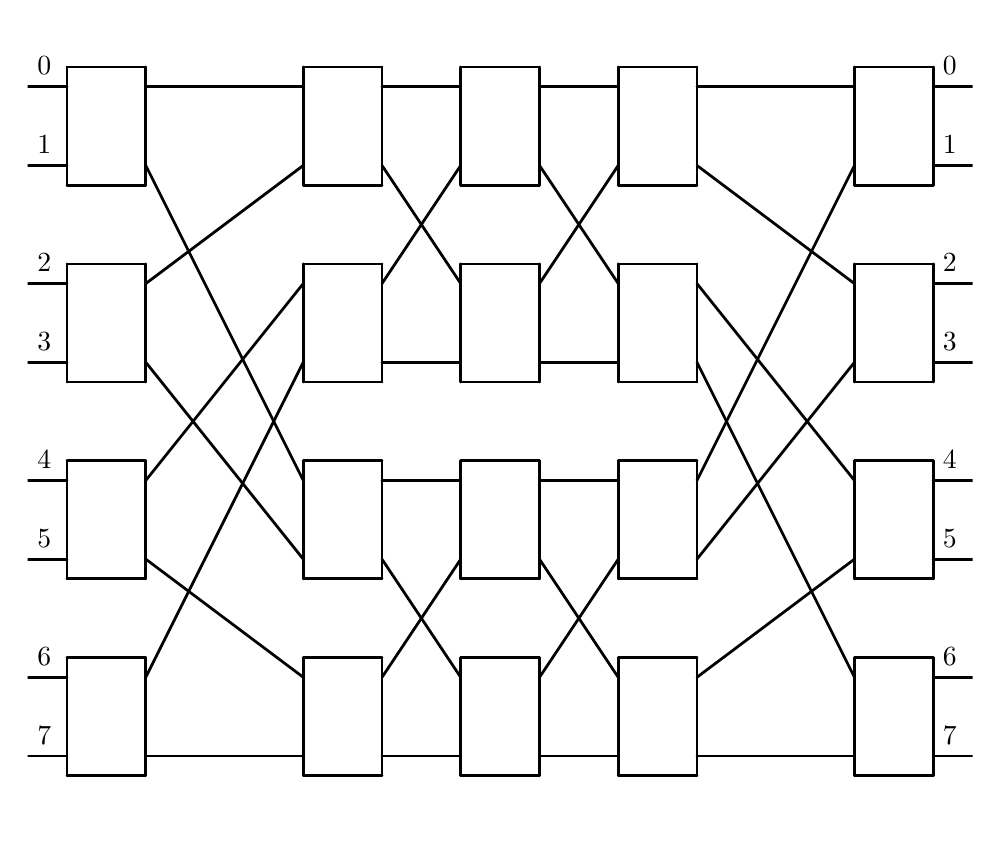
\begin{tikzpicture}[line cap=round,line join=round,>=triangle 45,x=0.5cm,y=0.5cm]
\clip(-7.,-1.) rectangle (17.,19.);
\draw [line width=1.pt] (0.,3.)-- (2.,3.);
\draw [line width=1.pt] (2.,3.)-- (2.,0.);
\draw [line width=1.pt] (2.,0.)-- (0.,0.);
\draw [line width=1.pt] (0.,0.)-- (0.,3.);
\draw [line width=1.pt] (0.,5.)-- (2.,5.);
\draw [line width=1.pt] (2.,5.)-- (2.,8.);
\draw [line width=1.pt] (2.,8.)-- (0.,8.);
\draw [line width=1.pt] (0.,8.)-- (0.,5.);
\draw [line width=1.pt] (4.,8.)-- (4.,5.);
\draw [line width=1.pt] (4.,5.)-- (6.,5.);
\draw [line width=1.pt] (6.,5.)-- (6.,8.);
\draw [line width=1.pt] (6.,8.)-- (4.,8.);
\draw [line width=1.pt] (4.,3.)-- (6.,3.);
\draw [line width=1.pt] (6.,3.)-- (6.,0.);
\draw [line width=1.pt] (6.,0.)-- (4.,0.);
\draw [line width=1.pt] (4.,0.)-- (4.,3.);
\draw [line width=1.pt] (8.,8.)-- (10.,8.);
\draw [line width=1.pt] (10.,8.)-- (10.,5.);
\draw [line width=1.pt] (10.,5.)-- (8.,5.);
\draw [line width=1.pt] (8.,5.)-- (8.,8.);
\draw [line width=1.pt] (8.,3.)-- (10.,3.);
\draw [line width=1.pt] (10.,3.)-- (10.,0.);
\draw [line width=1.pt] (10.,0.)-- (8.,0.);
\draw [line width=1.pt] (8.,0.)-- (8.,3.);
\draw [line width=1.pt] (2.,7.5)-- (4.,7.5);
\draw [line width=1.pt] (2.,5.5)-- (4.,2.5);
\draw [line width=1.pt] (2.,2.5)-- (4.,5.5);
\draw [line width=1.pt] (2.,0.5)-- (4.,0.5);
\draw [line width=1.pt] (6.,7.5)-- (8.,7.5);
\draw [line width=1.pt] (6.,5.5)-- (8.,2.5);
\draw [line width=1.pt] (6.,2.5)-- (8.,5.5);
\draw [line width=1.pt] (6.,0.5)-- (8.,0.5);
\draw [line width=1.pt] (0.,10.)-- (2.,10.);
\draw [line width=1.pt] (2.,10.)-- (2.,13.);
\draw [line width=1.pt] (2.,13.)-- (0.,13.);
\draw [line width=1.pt] (0.,13.)-- (0.,10.);
\draw [line width=1.pt] (4.,10.)-- (6.,10.);
\draw [line width=1.pt] (6.,10.)-- (6.,13.);
\draw [line width=1.pt] (6.,13.)-- (4.,13.);
\draw [line width=1.pt] (4.,13.)-- (4.,10.);
\draw [line width=1.pt] (8.,10.)-- (10.,10.);
\draw [line width=1.pt] (10.,10.)-- (10.,13.);
\draw [line width=1.pt] (10.,13.)-- (8.,13.);
\draw [line width=1.pt] (8.,13.)-- (8.,10.);
\draw [line width=1.pt] (4.,15.)-- (6.,15.);
\draw [line width=1.pt] (6.,15.)-- (6.,18.);
\draw [line width=1.pt] (6.,18.)-- (4.,18.);
\draw [line width=1.pt] (4.,18.)-- (4.,15.);
\draw [line width=1.pt] (8.,15.)-- (10.,15.);
\draw [line width=1.pt] (10.,15.)-- (10.,18.);
\draw [line width=1.pt] (10.,18.)-- (8.,18.);
\draw [line width=1.pt] (8.,18.)-- (8.,15.);
\draw [line width=1.pt] (2.,15.)-- (2.,18.);
\draw [line width=1.pt] (2.,18.)-- (0.,18.);
\draw [line width=1.pt] (0.,18.)-- (0.,15.);
\draw [line width=1.pt] (0.,15.)-- (2.,15.);
\draw [line width=1.pt] (2.,17.5)-- (4.,17.5);
\draw [line width=1.pt] (6.,17.5)-- (8.,17.5);
\draw [line width=1.pt] (2.,15.5)-- (4.,12.5);
\draw [line width=1.pt] (2.,12.5)-- (4.,15.5);
\draw [line width=1.pt] (2.,10.5)-- (4.,10.5);
\draw [line width=1.pt] (6.,12.5)-- (8.,15.5);
\draw [line width=1.pt] (6.,15.5)-- (8.,12.5);
\draw [line width=1.pt] (6.,10.5)-- (8.,10.5);
\draw [line width=1.pt] (-6.,18.)-- (-4.,18.);
\draw [line width=1.pt] (-4.,18.)-- (-4.,15.);
\draw [line width=1.pt] (-4.,15.)-- (-6.,15.);
\draw [line width=1.pt] (-6.,15.)-- (-6.,18.);
\draw [line width=1.pt] (-6.,13.)-- (-4.,13.);
\draw [line width=1.pt] (-4.,13.)-- (-4.,10.);
\draw [line width=1.pt] (-4.,10.)-- (-6.,10.);
\draw [line width=1.pt] (-6.,10.)-- (-6.,13.);
\draw [line width=1.pt] (-6.,8.)-- (-4.,8.);
\draw [line width=1.pt] (-4.,8.)-- (-4.,5.);
\draw [line width=1.pt] (-4.,5.)-- (-6.,5.);
\draw [line width=1.pt] (-6.,5.)-- (-6.,8.);
\draw [line width=1.pt] (-6.,3.)-- (-4.,3.);
\draw [line width=1.pt] (-4.,3.)-- (-4.,0.);
\draw [line width=1.pt] (-4.,0.)-- (-6.,0.);
\draw [line width=1.pt] (-6.,0.)-- (-6.,3.);
\draw [line width=1.pt] (14.,18.)-- (16.,18.);
\draw [line width=1.pt] (16.,18.)-- (16.,15.);
\draw [line width=1.pt] (16.,15.)-- (14.,15.);
\draw [line width=1.pt] (14.,15.)-- (14.,18.);
\draw [line width=1.pt] (14.,13.)-- (16.,13.);
\draw [line width=1.pt] (16.,13.)-- (16.,10.);
\draw [line width=1.pt] (16.,10.)-- (14.,10.);
\draw [line width=1.pt] (14.,10.)-- (14.,13.);
\draw [line width=1.pt] (14.,8.)-- (16.,8.);
\draw [line width=1.pt] (16.,8.)-- (16.,5.);
\draw [line width=1.pt] (16.,5.)-- (14.,5.);
\draw [line width=1.pt] (14.,5.)-- (14.,8.);
\draw [line width=1.pt] (14.,3.)-- (16.,3.);
\draw [line width=1.pt] (16.,3.)-- (16.,0.);
\draw [line width=1.pt] (16.,0.)-- (14.,0.);
\draw [line width=1.pt] (14.,0.)-- (14.,3.);
\draw [line width=1.pt] (-4.,17.5)-- (0.,17.5);
\draw [line width=1.pt] (-4.,15.5)-- (0.,7.5);
\draw [line width=1.pt] (-4.,12.5)-- (0.,15.5);
\draw [line width=1.pt] (-4.,10.5)-- (0.,5.5);
\draw [line width=1.pt] (-4.,7.5)-- (0.,12.5);
\draw [line width=1.pt] (-4.,5.5)-- (0.,2.5);
\draw [line width=1.pt] (-4.,2.5)-- (0.,10.5);
\draw [line width=1.pt] (-4.,0.5)-- (0.,0.5);
\draw [line width=1.pt] (14.,17.5)-- (10.,17.5);
\draw [line width=1.pt] (14.,15.5)-- (10.,7.5);
\draw [line width=1.pt] (14.,12.5)-- (10.,15.5);
\draw [line width=1.pt] (14.,10.5)-- (10.,5.5);
\draw [line width=1.pt] (14.,7.5)-- (10.,12.5);
\draw [line width=1.pt] (14.,5.5)-- (10.,2.5);
\draw [line width=1.pt] (14.,2.5)-- (10.,10.5);
\draw [line width=1.pt] (14.,0.5)-- (10.,0.5);
\draw [line width=1.pt] (-6.,17.5)-- (-7.,17.5);
\draw [line width=1.pt] (-6.,15.5)-- (-7.,15.5);
\draw [line width=1.pt] (-6.,12.5)-- (-7.,12.5);
\draw [line width=1.pt] (-6.,10.5)-- (-7.,10.5);
\draw [line width=1.pt] (-6.,7.5)-- (-7.,7.5);
\draw [line width=1.pt] (-6.,5.5)-- (-7.,5.5);
\draw [line width=1.pt] (-6.,2.5)-- (-7.,2.5);
\draw [line width=1.pt] (-6.,0.5)-- (-7.,0.5);
\draw [line width=1.pt] (16.,17.5)-- (17.,17.5);
\draw [line width=1.pt] (16.,15.5)-- (17.,15.5);
\draw [line width=1.pt] (16.,12.5)-- (17.,12.5);
\draw [line width=1.pt] (16.,10.5)-- (17.,10.5);
\draw [line width=1.pt] (16.,7.5)-- (17.,7.5);
\draw [line width=1.pt] (16.,5.5)-- (17.,5.5);
\draw [line width=1.pt] (16.,2.5)-- (17.,2.5);
\draw [line width=1.pt] (16.,0.5)-- (17.,0.5);
\draw (-7,18.5) node[anchor=north west] {0};
\draw (-7,16.5) node[anchor=north west] {1};
\draw (-7,13.5) node[anchor=north west] {2};
\draw (-7,11.5) node[anchor=north west] {3};
\draw (-7,8.5) node[anchor=north west] {4};
\draw (-7,6.5) node[anchor=north west] {5};
\draw (-7,3.5) node[anchor=north west] {6};
\draw (-7,1.5) node[anchor=north west] {7};
\draw (16,18.5) node[anchor=north west] {0};
\draw (16,16.5) node[anchor=north west] {1};
\draw (16,13.5) node[anchor=north west] {2};
\draw (16,11.5) node[anchor=north west] {3};
\draw (16,8.5) node[anchor=north west] {4};
\draw (16,6.5) node[anchor=north west] {5};
\draw (16,3.5) node[anchor=north west] {6};
\draw (16,1.5) node[anchor=north west] {7};
\end{tikzpicture}

\begin{minipage}{0.5\textwidth}
    \begin{center}
        {\it Sieć Beneša--Waksmana dla $n = 8$}
        
    \end{center}
\end{minipage}

\end{center}

\subsection{Optymalizacja}

Zauważmy, że można usunąć po jednym przełączniku na każdym rekurencyjnym poziomie sieci. Istotnie, w dowodzie powyżej ustaliliśmy \emph{dowolne} dwukolorowanie skonstruowanego grafu. Możemy jednak narzucić kolor wierzchołków w jednym przełączniku z warstwy wejściowej lub wyjściowej, np. ustalamy, że \(0 \in V_i\) ma kolor \emph{biały} oraz \(1 \in V_i\) ma kolor \emph{czarny}. Wówczas nie potrzebujemy zerowego przełącznika w warstwie wejściowej, gdyż możemy po prostu poprowadzić przewód z zerowego wejścia sieci do \emph{białej} podsieci oraz ten z pierwszego wejścia sieci do \emph{czarnej} podsieci. 

% --- Sieć realizująca wszystkie przesunięcia cykliczne ---

\section{Sieć realizująca wszystkie przesunięcia cykliczne}

Zastanówmy się teraz nad konstrukcją sieci, które realizują dowolne przesuniecie cykliczne. Dokładniej dla ustalonego \(n \in \N\) chcemy stworzyć sieć realizującą \(\lt\{ \shift n 0, \shift n 1, \ldots, \shift n {n-1} \rt\}\).

\begin{fa}\label{fa:zlozenie_shift}
    Dla dowolnych \(n, a, b \in \N\) zachodzi
    \[
    \shift n a \circ \shift n b = \shift n {a+b} \td
    \]
\end{fa}

\subsection{Konstrukcja i poprawność}

Skonstruujmy sieć w następujący sposób: złóżmy ze sobą sieci realizujące \({\shift n {2^0}, \shift n {2^1}, \ldots,}\) \(\shift n {2^k}\) dla \(k\), takiego że \(2^k < n\) (sieci z lematu \ref{lem:perm_shifty}). 

\begin{center}
    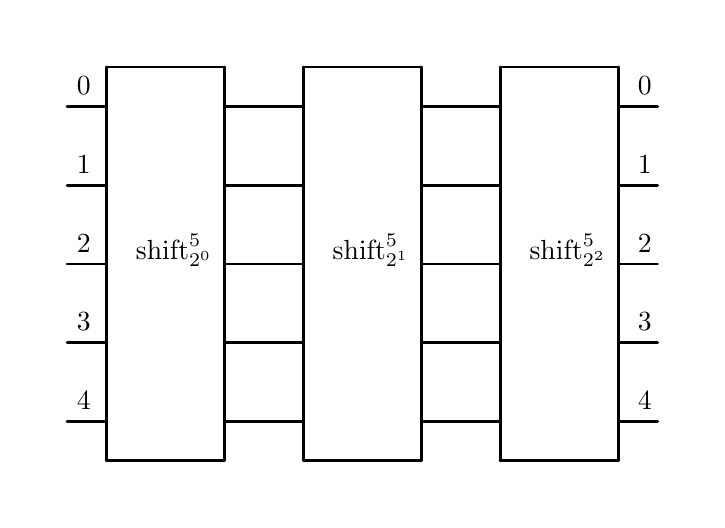
\begin{tikzpicture}[line cap=round,line join=round,>=triangle 45,x=0.5cm,y=0.5cm]
    \clip(-1.,-1.) rectangle (16.,11.);
    \draw [line width=1.pt] (1.,0.)-- (4.,0.);
    \draw [line width=1.pt] (4.,0.)-- (4.,10.);
    \draw [line width=1.pt] (4.,10.)-- (1.,10.);
    \draw [line width=1.pt] (1.,10.)-- (1.,0.);
    \draw [line width=1.pt] (0.,9.)-- (1.,9.);
    \draw [line width=1.pt] (1.,7.)-- (0.,7.);
    \draw [line width=1.pt] (1.,5.)-- (0.,5.);
    \draw [line width=1.pt] (1.,3.)-- (0.,3.);
    \draw [line width=1.pt] (1.,1.)-- (0.,1.);
    \draw [line width=1.pt] (6.,10.)-- (6.,0.);
    \draw [line width=1.pt] (6.,0.)-- (9.,0.);
    \draw [line width=1.pt] (6.,10.)-- (9.,10.);
    \draw [line width=1.pt] (9.,10.)-- (9.,0.);
    \draw [line width=1.pt] (11.,10.)-- (14.,10.);
    \draw [line width=1.pt] (11.,10.)-- (11.,0.);
    \draw [line width=1.pt] (11.,0.)-- (14.,0.);
    \draw [line width=1.pt] (14.,0.)-- (14.,10.);
    \draw [line width=1.pt] (4.,9.)-- (6.,9.);
    \draw [line width=1.pt] (4.,7.)-- (6.,7.);
    \draw [line width=1.pt] (4.,5.)-- (6.,5.);
    \draw [line width=1.pt] (4.,3.)-- (6.,3.);
    \draw [line width=1.pt] (4.,1.)-- (6.,1.);
    \draw [line width=1.pt] (9.,9.)-- (11.,9.);
    \draw [line width=1.pt] (9.,7.)-- (11.,7.);
    \draw [line width=1.pt] (9.,5.)-- (11.,5.);
    \draw [line width=1.pt] (9.,3.)-- (11.,3.);
    \draw [line width=1.pt] (9.,1.)-- (11.,1.);
    \draw (1.5, 6) node[anchor=north west] {$\shift 5 {2^0}$};
    \draw (6.5, 6) node[anchor=north west] {$\shift 5 {2^1}$};
    \draw (11.5,6) node[anchor=north west] {$\shift 5 {2^2}$};
    \draw [line width=1.pt] (14.,9.)-- (15.,9.);
    \draw [line width=1.pt] (14.,7.)-- (15.,7.);
    \draw [line width=1.pt] (14.,5.)-- (15.,5.);
    \draw [line width=1.pt] (14.,3.)-- (15.,3.);
    \draw [line width=1.pt] (14.,1.)-- (15.,1.);
    \draw (0, 10) node[anchor=north west] {0};
    \draw (0, 8)  node[anchor=north west] {1};
    \draw (0, 6)  node[anchor=north west] {2};
    \draw (0, 4)  node[anchor=north west] {3};
    \draw (0, 2)  node[anchor=north west] {4};
    \draw (14.25, 10) node[anchor=north west] {0};
    \draw (14.25, 8)  node[anchor=north west] {1};
    \draw (14.25, 6)  node[anchor=north west] {2};
    \draw (14.25, 4)  node[anchor=north west] {3};
    \draw (14.25, 2)  node[anchor=north west] {4};
    \end{tikzpicture}
    
    \begin{minipage}{0.5\textwidth}
        \begin{center}
            {\it Schemat sieci realizującej wszystkie przesunięcia cykliczne zbioru 5-elementowego}
        \end{center}
    \end{minipage}
    \end{center}

\vspace{.5em}

Ustalmy teraz \(j \in \lt\{ 0, 1, \ldots, n-1 \rt\}\). Aby zrealizować \(\shift n j\) należy aktywować sieci realizujące \(\shift n {2^l}\), takie że na \(l\)--tej pozycji w zapisie binarnym \(j\) występuje jedynka. Z  faktu \ref{fa:zlozenie_shift} wynika, że w ten sposób zrealizujemy \(\shift n j\). 

\subsection{Rozmiar i głębokość}

Zauważmy, że stwarzamy \(\Theta(\log n)\) podsieci, a każda z nich ma rozmiar  \(\floor{\frac n 2}\) i głębokość 1. Wobec tego rozmiar skonstruowanej sieci wynosi \(\Theta(n \log n)\), a głębokość \(\Theta(\log n)\).

% -- Sieć realizująca przesunięcia cykliczne o potęgi 2 ---

\section{Sieć realizująca przesunięcia cykliczne o potęgi 2}

W tym rozdziale chcemy zastanowić się nad konstrukcją sieci o \(n\) wejściach i \(n\) wyjściach realizującej przesunięcia cykliczne o potęgi 2 nie większe niż \(n\), to znaczy chcemy zrealizować zbiór

\[
\twoshift{n} = \{ \id n \tc \shift n {2^0} \tc \shift n {2^1} \tc \ldots \shift n {2^l}\} \tc
\]

gdzie \(2^l \leq n\) oraz \(2^{l+1} > n\). Dla uproszczenia przyjmiemy, że \(n = 2^{2^r}\) dla pewnego \(r \in \N\) i oznaczymy \( m = \sqrt{n} = 2^{2^{r-1}} \). Uogólnienie konstrukcji dla dowolnego \(n \in \N\) zostało przedstawione w \cite{klo}.

% \vspace{1em}

\subsection{Zmiana sposobu reprezentacji ciągu}

W tym rozdziale będziemy wyobrażać sobie zbiór \(\{0, 1, 2, \ldots, n-1\}\) jako macierz o wymiarach \(m \times m\) -- to uzasadnia wybór \(n\), które jest kwadratem liczby naturalnej. Na przykład dla \(r = 2\) mamy \(n = 2^{2^2} = 2^4 = 16\), a macierzowa reprezentacja zbioru wygląda następująco:
\[
\begin{matrix}
 0 &  1 &  2 &  3 \\
 4 &  5 &  6 &  7 \\
 8 &  9 & 10 & 11 \\
12 & 13 & 14 & 15
\end{matrix}
\]

Zastanówmy się teraz, jak wyglądają przesunięcia cykliczne o \(2^k\) w tej reprezentacji.

\subsection{Przesunięcia cykliczne o duże \(2^k\)}

 Gdy \(2^k\) jest \textit{duże}, to znaczy \(2^k \geq m\) (równoważnie \(k \geq 2^{r-1}\)), to \(m \, | \, 2^k\). Wobec tego \(\shift n {2^k}\) jest przesunięciem cyklicznym o \(2^k / m = 2^k / 2^{2^{r-1}} = 2^{k - 2^{r-1}}\) na zbiorze wierszy. Na przykład dla \(n = 64 = 2^{2^3}\) oraz \(2^k = 2^4 = 2 \cdot \sqrt{64}\) mamy

\vspace{0.5em}

\begin{minipage}{.5\textwidth} %

\[
\begin{matrix}
 0 &  1 &  2 &  \ldots & 7 \\
 8 &  9 & 10 &  \ldots & 15 \\
\ldots & & \ddots &  & \vdots \\
48 & 49 & 50 & \ldots & 55 \\
56 & 57 & 58 & \ldots & 63 
\end{matrix}
\]

\begin{center} \it
    Zbiór przed wykonaniem \(\shift {64} {16}\).
\end{center}

\end{minipage} %
\begin{minipage}{.5\textwidth} %

\[
\begin{matrix}
16 & 17 & 18 & \ldots & 23 \\
24 & 25 & 26 & \ldots & 31 \\
\ldots & & \ddots &  & \vdots \\
56 & 57 & 58 & \ldots & 63 \\
0 &  1 &  2 &  \ldots & 7 \\
8 &  9 & 10 &  \ldots & 15 \\
\end{matrix}
\]

\begin{center} \it
    Zbiór po wykonaniu \(\shift {64} {16}\).
\end{center}
\end{minipage}

\vspace{1em}

Możemy także pomyśleć o tym nieco inaczej. Dokładniej, \(\shift n {2^k}\) może być wykonany w 3 etapach:

\begin{enumerate}
    \item transpozycja macierzy,
    \item \(\shift {m} {2^k/m}\) na wierszach tak otrzymanej macierzy,
    \item transpozycja macierzy.
\end{enumerate}

Przeanalizujmy to na powyższym przykładzie -- \(n = 64\) oraz \(2^k = 16\).

\vspace{0.5em}

\begin{minipage}{.5\textwidth} %

\[
\begin{matrix}
 0 &  1 &  2 &  \ldots & 7 \\
 8 &  9 & 10 &  \ldots & 15 \\
\ldots & & \ddots &  & \vdots \\
48 & 49 & 50 & \ldots & 55 \\
56 & 57 & 58 & \ldots & 63 
\end{matrix}
\]

\begin{center} \it
    Początkowy zbiór.
\end{center}

\end{minipage} %
\begin{minipage}{.5\textwidth} %

\[
\begin{matrix}
 0 &  8 &  16 &  \ldots & 56 \\
 1 &  9 &  17 &  \ldots & 57 \\
\ldots  & & \ddots &     & \vdots \\
 6 & 14 & 22 & \ldots   & 62 \\
 7 & 15 & 23 & \ldots   & 63 
\end{matrix}
\]

\begin{center} \it
    Zbiór po wykonaniu transpozycji.
\end{center}
\end{minipage}

\vspace{0.5em}

\begin{minipage}{.5\textwidth} %
\[
\begin{matrix}
 16 &  24 &  \ldots & 0 & 8 \\
 17 &  25 &  \ldots & 1 & 9 \\
\ldots  & &  \ddots &   & \vdots \\
 22 &  30 &  \ldots & 6 & 14 \\
 23 &  31 &  \ldots & 7 & 15
\end{matrix}
\]

\begin{center} \it
    Zbiór po wykonaniu \(\shift{8}{2}\) na wierszach macierzy.
\end{center}

\end{minipage} %
\begin{minipage}{.5\textwidth} %

\[
\begin{matrix}
 16 &  17 &  \ldots & 22 & 23 \\
 24 &  25 &  \ldots & 30 & 31 \\
\ldots  & &  \ddots &    & \vdots \\
  0 &   1 &  \ldots &  6 & 7 \\
  8 &   9 &  \ldots &  14 & 15
\end{matrix}
\]

\begin{center} \it
    Zbiór po wykonaniu transpozycji.
\end{center}
\end{minipage}

\subsection{Przesunięcia cykliczne o małe \(2^k\)}

Co się dzieje, gdy \(2^k\) jest \textit{małe} (to znaczy \(2^k < m \))? Wtedy zmiany w układzie liczb zachodzą także wewnątrz wierszy. Istotnie -- \(\shift n {2^k}\) możemy wówczas przedstawić jako dwa etapy:
\begin{enumerate}
    \item \(\shift{m}{2^k}\) wewnątrz każdego wiersza,
    \item \(\shift{m}{1}\) wewnątrz ostatnich \(2^k\) kolumn.
\end{enumerate}

Przyjrzyjmy się tym etapom na przykładzie -- niech \(n=64\) oraz \(2^k = 2\).

\vspace{0.5em}

\begin{minipage}{.5\textwidth} %

\[
\begin{matrix}
 0 &  1 &  2 &  \ldots & 7 \\
 8 &  9 & 10 &  \ldots & 15 \\
\ldots & & \ddots &  & \vdots \\
48 & 49 & 50 & \ldots & 55 \\
56 & 57 & 58 & \ldots & 63 
\end{matrix}
\]

\begin{center} \it
    Początkowy zbiór.
\end{center}

\end{minipage} %
\begin{minipage}{.5\textwidth} %

\[
\begin{matrix}
 2  &  3 & \ldots &  0 &  1 \\
 10 & 11 & \ldots &  8 &  9 \\
\ldots & & \ddots &  & \vdots \\
 50 & 51 & \ldots & 48 & 49 \\
 58 & 59 & \ldots & 56 & 57 \\ 
\end{matrix}
\]

\begin{center} \it
    Zbiór po wykonaniu \(\shift 8 2\) na każdym wierszu.
\end{center}
\end{minipage}

\vspace{1em}

\begin{minipage}{.5\textwidth} %

\[
\begin{array}{c c  c c}
 2  &  3 & \ldots & 7 \\
 10 & 11 & \ldots & 15 \\
\ldots & & \ddots &  \vdots \\
 50 & 51 & \ldots & 56  \\
 58 & 59 & \ldots & 63  \\ 
\end{array}
\begin{array}{| c c |}
\hline
 0 &  1 \\
 8 &  9 \\
\vdots & \vdots \\
 48 & 49 \\
 56 & 57 \\
 \hline
\end{array}
\]

\begin{center} \it
    Kolumny, na których należy wykonać \(\shift 8 1\).
\end{center}
\end{minipage}
\begin{minipage}{.5\textwidth} %

\[
\begin{matrix}
 2  &  3 & \ldots & 8  &  9  \\
 10 & 11 & \ldots & 16 & 17\\
\ldots & & \ddots &  & \vdots \\
 50 & 51 & \ldots & 56 & 57 \\
 58 & 59 & \ldots & 0 &  1 \\ 
\end{matrix}
\]

\begin{center} \it
    Zbiór po wykonaniu \(\shift 8 1\) na 2 ostatnich kolumnach.
\end{center}
\end{minipage}

% \vspace{1em}

\subsection{Konstrukcja sieci}

Podsumowując, przesunięcia cykliczne o \(2^k\) realizujemy w następujący sposób:

\begin{itemize}
    \item gdy \(2^k\) jest małe, wykonujemy \(\shift{m}{2^k}\) wewnątrz każdego wiersza, a następnie \(\shift{m}{1}\) wewnątrz ostatnich \(2^k\) kolumn,
    \item gdy \(2^k\) jest duże, transponujemy macierz, wykonujemy \(\shift {m} {2^k/m} \) na wierszach i znowu transponujemy macierz.
\end{itemize}

To pozwala już sformułować przybliżoną konstrukcję sieci. Aby skonstruować \(P_n\) -- sieć realizującą \(\twoshift n\), potrzebujemy następujących podsieci (zwanych dalej \textit{blokami}):

\begin{itemize}
    \item sieci realizującej transpozycję i \(\id n\) (oznaczmy ją \(T_1\)),
    \item \(m\) sieci realizujących \( \twoshift m\) -- czyli \(m\) kopii sieci \(P_m\) (nazwijmy je \textit{blokiem wierszowym}),
    \item \(m\) sieci realizujących \(\shift m 1\) oraz \(\id m\) dla każdej kolumny, takich jak w lemacie \ref{lem:perm_shifty} -- nazwijmy je \textit{blokiem kolumnowym}
    \item oraz drugiej sieci realizującej transpozycję i \(\id n\) (oznaczmy ją \(T_2\)).
\end{itemize}


Oczywiście transpozycja jest inwolucją -- w związku z tym sieci \(T_1\) i \(T_2\) mogą zostać utworzone tak jak w lemacie \ref{lem:perm_inwolucje}. 
W terminach tak skonstruowanej sieci zrealizowanie przesunięcia cyklicznego o \(2^k\) wygląda następująco:

\begin{itemize}
    \item gdy \(2^k\) jest małe, aktywujemy blok wierszowy, tak by wykonał \(\shift m {2^k}\) na każdym wierszu, a następnie aktywujemy blok kolumnowy, tak by wykonał \(\shift m 1\) na ostatnich \(2^k\) kolumnach,
    \item gdy \(2^k\) jest duże, aktywujemy sieć \(T_1\), tak by wykonała transpozycję, aktywujemy blok wierszowy, tak by wykonał \(\shift m {2^k/m}\) na każdym wierszu, a na końcu aktywujemy aktywujemy sieć \(T_2\), tak by wykonała transpozycję.
\end{itemize}

\subsection{Głębokość i rozmiar}

Udało nam się skonstruować sieć realizującą \(\twoshift n\). Zbadajmy teraz jej głębokość i rozmiar.

\begin{lem}
    Sieć przedstawiona wyżej ma głębokość równą \(D(n) = \Theta(\log \log n)\).
\end{lem}

\begin{proof}
    Zauważmy, że zarówno blok \(T_1\), jaki i blok \(T_2\), mają głębokość równą 1. Blok kolumnowy ma głębokość równą 2, a blok wierszowy -- \(D(m) = D(\sqrt{n})\). Wobec tego głębokość sieci wyraża się następującym równaniem rekurencyjnym:
    \[
    D(n) = D(\sqrt n) + O(1) \td
    \]
    Do rozwiązania tej rekurencji zastosujemy metodę podstawiania. Niech \(s = \log n\). Mamy wówczas
    \[
    D(2^s) = D(2^{s/2}) + O(1) \td
    \]
    Oznaczmy \(B(s) = D(2^s)\). Dla \(B\) rekurencja przedstawia się następująco:
    \[
    B(s) = B\left(\frac s 2\right) + O(1) \td
    \]
    Na mocy twierdzenia o rekurencji uniwersalnej (ang. \textit{master theorem}, \cite{cormen}) otrzymujemy
    \[
    B(s) = \Theta(\log s) \tc
    \]
    a zapisując powyższą równość w terminach \(D\), dostajemy
    \[
    D(n) = D(2^s) = B(s) = \Theta(\log s) = \Theta(\log \log n) \td
    \]
\end{proof}

\begin{lem}
    Sieć przedstawiona wyżej ma rozmiar równy \(S(n) = \Theta(n \log \log n)\). 
\end{lem}

\begin{proof}
    Zauważmy, że sieci \(T_1\) i \(T_2\) mają rozmiar równy \( \floor{\frac{n - \sqrt{n}}{2}} \). Ponadto rozmiar całego bloku kolumnowego wynosi co najwyżej \(m \cdot \frac{m}{2} \cdot 2\), gdzie \(m = \sqrt{n}\), a rozmiar bloku wierszowego to \(mS(m)\).  Otrzymujemy zatem następujące równanie rekurencyjne
    \[
    S(n) = 2 \cdot \floor{\frac{n - \sqrt{n}}{2}} + O\left(\sqrt{n} \cdot \frac{\sqrt{n}}{2} \cdot 2\right) + \sqrt{n}S(\sqrt{n})
    = \sqrt{n}S(\sqrt{n}) + \Theta(n) \td
    \]
    Przypomnijmy, że \(n = 2^{2^r}\).  Mamy zatem równoważnie
    \begin{align*}
         S \lt( 2^{2^r} \rt) 
         &= 2^{2^{r-1}} S \lt( 2^{2^{r-1}} \rt) + \Theta \lt( 2^{2^r} \rt) \\
         &= 2^{2^{r-1}} \lt( 2^{2^{r-2}} S \lt( 2^{2^{r-2}} \rt) + \Theta \lt( 2^{2^{r-1}} \rt) \rt) + \Theta \lt( 2^{2^r} \rt) \\
         &= 2^{2^{r-1} + 2^{r-2}} S \lt( 2^{2^{r-2}} \rt)
         + 2^{2^{r-1}} \Theta \lt( 2^{2^{r-1}} \rt) + \Theta \lt( 2^{2^{r}} \rt) \\
         &= 2^{2^{r-1} + 2^{r-2}} S \lt( 2^{2^{r-2}} \rt)
         + \Theta \lt( 2^{2^{r}} \rt) + \Theta \lt( 2^{2^{r}} \rt) \\
         &= 2^{2^{r-1} + 2^{r-2}}  \lt( 2^{2^{r-3}} S \lt( 2^{2^{r-3}} \rt) + \Theta \lt( 2^{2^{r-2}} \rt)  \rt)
         + \Theta \lt( 2^{2^{r}} \rt) + \Theta \lt( 2^{2^{r}} \rt) \\
         &=  2^{2^{r-1} + 2^{r-2} + 2^{r-3}} S \lt( 2^{2^{r-3}} \rt)  + \Theta \lt( 2^{2^{r}} \rt) + \Theta \lt( 2^{2^{r}} \rt) + \Theta \lt( 2^{2^{r}} \rt) \\
         &= \ldots \\
         &=  2^{2^{r-1} + 2^{r-2} + \ldots + 2^{0}} S \lt( 2^{2^{0}} \rt) + r \Theta \lt( 2^{2^{r}} \rt) \\
         &= 2^{2^{r}-1} S \lt( 2^{2^{0}} \rt) + \Theta \lt( r2^{2^{r}} \rt) \\
         &= \Theta \lt( 2^{2^{r}} \rt) + \Theta \lt( r 2^{2^{r}} \rt) = \Theta \lt( r2^{2^{r}} \rt)
    \end{align*}
   
    Intuicyjnie: widzimy, że wykładnik wykładnika maleje o 1 w zależności rekurencyjnej. Wobec tego jeśli będziemy iterować wstawianie zależności rekurencyjnej do prawej strony równania, wykonamy \(r\) iteracji, a każda dołoży do ostatecznej sumy składnik \( \Theta \lt( 2^{2^{r}} \rt) \).

    \vspace{1em}

    Podstawiając \(n = 2^{2^r}\) do otrzymanej równości, otrzymujemy
    \[
    S(n) = \Theta(n \log \log n) \td
    \]
    
\end{proof}


% % ------------------ Co dalej? -------------------

% \section{Co dalej?}

% Losowe ustawianie przełączników -- analiza probabilistyczna. 

% ------------- bibliografia ----------------------

\begin{thebibliography}{9}
\bibitem{klo}
Juraj Hromkovič, Przemyslawa Kanarek, Ralf Klasing, Krzysztof Lorys, Walter Unger, et al.. \emph{On the Size of Permutation Networks and Consequences for Efficient Simulation of Hypercube Algorithms on Bounded-Degree Networks}. SIAM Journal on Discrete Mathematics, 2009, 23 (3), pp.1612–1645. ff10.1137/060669164ff. ffhal-00402764f

\bibitem{cormen}
Thomas H. Cormen, Charles E. Leiserson, Ronald L. Rivest, Clifford Stein, \emph{Introduction to Algorithms}, The MIT Press, 2022
\end{thebibliography}

\end{document}